% =============================================================================
%  EduSoundMetrics - Memoria de Investigacion
%  Documento unificado: Volumen I (Memoria) + Volumen II (Documentacion tecnica)
%  Compilar con: pdflatex -shell-escape memoria_investigacion.tex (x2 + biber si)
% =============================================================================

\documentclass[11pt,a4paper,openany]{report}

% ----- PAQUETES ESENCIALES -----
\usepackage[utf8]{inputenc}
\usepackage[T1]{fontenc}
\usepackage{lmodern}
\usepackage[spanish,es-tabla,es-noshorthands]{babel}
\usepackage{amsmath}
\usepackage{graphicx}
\usepackage[table]{xcolor}
\usepackage{geometry}
\usepackage{booktabs}
\usepackage{tabularx}
\usepackage{titlesec}
\usepackage{fancyhdr}
\usepackage{enumitem}
\usepackage{float}
\usepackage{caption}
\usepackage[skins,breakable]{tcolorbox}
\usepackage{hyperref}
\usepackage{fontawesome5}
\usepackage{parskip}
\usepackage{listings}
\usepackage{tikz}
\usetikzlibrary{shapes,arrows.meta,positioning,fit,backgrounds,patterns,calc}
\usepackage{pgfplots}
\pgfplotsset{compat=1.18}
\usepackage{eurosym}
\usepackage{textcomp}

\renewcommand{\familydefault}{\sfdefault}
\geometry{top=2.5cm, bottom=2.5cm, left=2.5cm, right=2.5cm, headheight=24pt}

% ----- PALETA -----
\definecolor{CorpDark}{HTML}{0F172A}
\definecolor{CorpBlue}{HTML}{2563EB}
\definecolor{CorpAccent}{HTML}{F97316}
\definecolor{BgGray}{HTML}{F8FAFC}
\definecolor{TableHead}{HTML}{E2E8F0}
\definecolor{dbgreen}{HTML}{22c55e}
\definecolor{dbyellow}{HTML}{eab308}
\definecolor{dbred}{HTML}{ef4444}
\definecolor{codegreen}{rgb}{0.0, 0.5, 0.0}
\definecolor{codegray}{rgb}{0.5, 0.5, 0.5}
\definecolor{codepurple}{rgb}{0.58, 0.0, 0.82}
\definecolor{backcolour}{rgb}{0.97, 0.97, 0.97}

% ----- HYPERREF -----
\hypersetup{
    colorlinks=true,
    linkcolor=CorpDark,
    urlcolor=CorpBlue,
    citecolor=CorpBlue,
    pdftitle={EduSoundMetrics - Memoria de Investigacion},
    pdfauthor={CPIFP Los Enlaces}
}

% ----- TITULOS -----
\titleformat{\part}[display]
  {\centering\color{CorpDark}\Huge\bfseries}
  {\color{CorpAccent}\Large VOLUMEN \thepart}{1em}{}
\titleformat{\chapter}[hang]
  {\color{CorpDark}\huge\bfseries}
  {\color{CorpBlue}\thechapter.}{0.5em}{}
  [\vspace{-0.2cm}\color{CorpBlue}\titlerule\vspace{0.3cm}]
\titleformat{\section}
  {\color{CorpDark}\Large\bfseries}
  {\color{CorpBlue}\thesection.}{0.7em}{}
\titleformat{\subsection}
  {\color{CorpDark}\large\bfseries}
  {\color{CorpAccent}\thesubsection.}{0.7em}{}
\titleformat{\subsubsection}
  {\color{CorpDark}\normalsize\bfseries}
  {\thesubsubsection.}{0.7em}{}

% ----- CAJAS -----
\newtcolorbox{InfoBox}[1][]{
    enhanced, breakable, colback=BgGray, colframe=CorpBlue, boxrule=1pt,
    arc=4pt, left=15pt, right=15pt, top=10pt, bottom=10pt,
    drop fuzzy shadow, fonttitle=\bfseries\large, title=#1
}
\newtcolorbox{HighlightBox}{
    enhanced, breakable, colback=CorpBlue!5!white, colframe=CorpBlue,
    borderline west={4pt}{0pt}{CorpBlue}, sharp corners,
    boxrule=0pt, left=15pt, right=15pt, top=10pt, bottom=10pt
}
\newtcolorbox{KeyFinding}{
    enhanced, breakable, colback=CorpAccent!10, colframe=CorpAccent,
    borderline west={4pt}{0pt}{CorpAccent}, sharp corners,
    boxrule=0pt, left=15pt, right=15pt, top=10pt, bottom=10pt
}

% ----- LISTINGS -----
\lstdefinestyle{code}{
    backgroundcolor=\color{backcolour},
    commentstyle=\color{codegreen},
    keywordstyle=\color{codepurple}\bfseries,
    numberstyle=\tiny\color{codegray},
    stringstyle=\color{red!70!black},
    basicstyle=\ttfamily\footnotesize,
    breakatwhitespace=false, breaklines=true, captionpos=b,
    keepspaces=true, numbers=left, numbersep=8pt,
    showspaces=false, showstringspaces=false, showtabs=false,
    tabsize=2, frame=single, rulecolor=\color{gray!30},
    xleftmargin=1.5em, framexleftmargin=1.5em,
}
\lstset{style=code}

% ----- HEADERS -----
\pagestyle{fancy}
\fancyhf{}
\renewcommand{\headrulewidth}{0.5pt}
\renewcommand{\headrule}{\hbox to\headwidth{\color{CorpBlue}\leaders\hrule height \headrulewidth\hfill}}
\lhead{\color{CorpDark}\textbf{EduSoundMetrics} | Memoria de Investigacion}
\rhead{\color{CorpDark}CPIFP Los Enlaces}
\cfoot{\color{CorpDark}\textbf{\thepage}}
\renewcommand{\chaptermark}[1]{\markboth{\thechapter.\ #1}{}}

% =============================================================================
\begin{document}

% =============================================================================
% PORTADA
% =============================================================================
\begin{titlepage}
    \pagecolor{CorpDark}
    \color{white}
    \centering
    \vspace*{1.5cm}

    {\Huge\textcolor{CorpAccent}{\faBroadcastTower}}\par
    \vspace{0.8cm}
    {\scshape\Large CPIFP Los Enlaces \par}
    \vspace{0.3cm}
    {\large Departamento de Inform\'atica y Comunicaciones\par}
    \vspace{2cm}

    {\Huge\bfseries EDUSOUND METRICS \par}
    \vspace{0.4cm}
    {\Large Sistema Distribuido de Monitorizaci\'on Ac\'ustica IoT \\ para Espacios Educativos \par}
    \vspace{0.6cm}
    {\large \textit{Monitor de Ruido en Aulas} \par}

    \vspace{2cm}
    \begin{tcolorbox}[
        colback=CorpDark!80!black,
        colframe=CorpBlue,
        coltext=white,
        width=0.88\textwidth,
        center, arc=8pt, boxrule=1.5pt, boxsep=10pt
    ]
        \centering
        \Large\textbf{Memoria de Investigaci\'on}\\[0.2cm]
        \normalsize
        \textit{Estudio comparativo de arquitecturas de monitorizaci\'on ac\'ustica IoT en un aula testigo}\\[0.4cm]
        \large
        \textcolor{CorpAccent}{\textbf{Volumen I:}} Investigaci\'on, metodolog\'ia y resultados\\[0.15cm]
        \textcolor{CorpAccent}{\textbf{Volumen II:}} Arquitectura t\'ecnica y despliegue
    \end{tcolorbox}

    \vspace{1.2cm}
    \begin{tabular}{rl}
    \textcolor{CorpAccent}{\textbf{Pregunta de investigaci\'on:}} &
        \begin{minipage}[t]{0.6\textwidth}
            \emph{¿Aporta una malla de 6 micr\'ofonos perimetrales informaci\'on suficientemente superior a un \'unico nodo central como para justificar su mayor coste e instalaci\'on?}
        \end{minipage}\\[0.4cm]
    \textcolor{CorpAccent}{\textbf{Aula piloto:}} & DAM (turno ma\~nana) / SMR (turno tarde) \\[0.2cm]
    \textcolor{CorpAccent}{\textbf{Periodo de medici\'on:}} & 20 abril -- 04 mayo 2026 \\[0.2cm]
    \textcolor{CorpAccent}{\textbf{Repositorio:}} & \texttt{github.com/Rubenbros/microfonoAula} \\
    \end{tabular}

    \vfill
    {\large Zaragoza, \today \par}
\end{titlepage}
\nopagecolor
\thispagestyle{empty}

% =============================================================================
% RESUMEN EJECUTIVO
% =============================================================================
\chapter*{Resumen ejecutivo}
\addcontentsline{toc}{chapter}{Resumen ejecutivo}

\textbf{EduSoundMetrics} es un sistema distribuido de monitorizaci\'on ac\'ustica IoT desarrollado en el CPIFP Los Enlaces para evaluar empíricamente qu\'e arquitectura es m\'as adecuada para vigilar el confort sonoro en un aula educativa: una \emph{malla} de 6 micr\'ofonos perimetrales, un \emph{nodo central} \'unico, o ambos en convivencia. Para responder a esa pregunta se ha desplegado una instalaci\'on completa en un aula piloto compartida por los ciclos de DAM (turno de ma\~nana) y SMR (turno de tarde).

\begin{KeyFinding}
\textbf{\faChartBar\ Hallazgos clave del piloto (657.549 lecturas, 14 d\'ias)}
\begin{itemize}[leftmargin=1.2em]
    \item El aula opera de manera predominantemente silenciosa: el \textbf{94,1\,\%} de las lecturas est\'an por debajo de 50\,dB(A) y solo el \textbf{0,002\,\%} supera los 70\,dB(A).
    \item El nodo central (\texttt{mic\_central}) presenta un sesgo posicional de \textbf{+10,9\,dB(A)} sin calibrar respecto a la mediana de los distribuidos. La calibraci\'on en backend (\texttt{$-7$\,dB}) reduce ese sesgo a \textbf{+3,9\,dB(A)} residuales, absorbidos por la agregaci\'on por mediana.
    \item El turno de ma\~nana (DAM) registra una media de \textbf{39,3\,dB(A)} frente a los \textbf{35,9\,dB(A)} del turno de tarde (SMR), una diferencia de \textbf{+3,4\,dB(A)} pondrada por horas lectivas.
    \item La validaci\'on bipolar por extremos (silencio nocturno + est\'imulo controlado) es coherente con la literatura: \textbf{$\approx$\,21\,dB(A)} de suelo nocturno y picos de hasta \textbf{84,6\,dB(A)} en el ensayo del 27/04/2026.
    \item La \textbf{mediana espacial} sobre 7 micros se demuestra robusta frente al outlier posicional del central, evitando la sobre-estimaci\'on que producir\'ia la media aritm\'etica.
\end{itemize}
\end{KeyFinding}

\textbf{Recomendaci\'on}: para despliegues institucionales masivos, el nodo central (M5Stack Core2) ofrece la mejor relaci\'on coste/valor anal\'itico al entregar la mayor parte de la informaci\'on \'util con un \'unico punto de instalaci\'on. La malla de 6 nodos aporta granularidad espacial relevante \'unicamente para escenarios de investigaci\'on o aulas de geometr\'ia compleja, y se mantiene como infraestructura demostradora del piloto. Esta recomendaci\'on, justificada en la \S\,\ref{sec:discusion-arq}, est\'a sujeta a la limitaci\'on de haber sido validada en una sola aula durante 14 d\'ias.

\newpage

% =============================================================================
% INDICE
% =============================================================================
\tableofcontents
\newpage

% #############################################################################
% PARTE I --- MEMORIA DE INVESTIGACION
% #############################################################################
\part{Memoria de investigaci\'on}

\chapter{Introducci\'on y planteamiento}

\section{Contexto educativo y motivaci\'on}

El paradigma educativo de la Formaci\'on Profesional actual exige metodolog\'ias activas, aprendizaje basado en proyectos (ABP) y trabajo colaborativo. Estas din\'amicas, esenciales para la adquisici\'on de competencias profesionales, conllevan inevitablemente un aumento de la presi\'on ac\'ustica en las aulas, lo que puede deteriorar el clima de aprendizaje, la concentraci\'on y la salud laboral del profesorado.

A diferencia de los entornos industriales, donde el control del ruido cuenta con una infraestructura de medici\'on consolidada, en las aulas educativas los datos cuantitativos son escasos y la decisi\'on sobre c\'omo y cu\'anto medir queda habitualmente en manos del personal docente sin herramientas espec\'ificas. EduSoundMetrics nace para colmar esta laguna en el centro mediante un sistema IoT propio, replicable y de bajo coste.

\section{Justificaci\'on normativa y te\'orica}

El control del confort ac\'ustico no es \'unicamente una cuesti\'on de comodidad, sino un imperativo de salud p\'ublica y rendimiento cognitivo avalado por la literatura cient\'ifica:

\begin{HighlightBox}
\textbf{\faBook\ Marco cient\'ifico y est\'andares de calidad}\\[0.2em]
\textbf{1. Organizaci\'on Mundial de la Salud (OMS, 2018):} Niveles de exposici\'on continua superiores a $55$\,dB en entornos de concentraci\'on afectan negativamente a la memoria a corto plazo y elevan los niveles de cortisol en estudiantes y docentes.\\[0.2em]
\textbf{2. ISO 9241-6 (Ergonom\'ia del entorno de trabajo):} Las tareas que requieren alta concentraci\'on intelectual --como las pr\'acticas de programaci\'on o sistemas-- requieren un ruido de fondo m\'aximo de \textbf{45 a 55\,dB}.\\[0.2em]
\textbf{3. IEC 61672 (Sonometr\'ia clase 1 y 2):} Define la curva de ponderaci\'on A (dBA) que reproduce la sensibilidad del o\'ido humano. Es el est\'andar internacional para medici\'on de ruido ambiental.
\end{HighlightBox}

\section{Pregunta de investigaci\'on}

El proyecto se plantea como objetivo investigador resolver de forma emp\'irica la siguiente pregunta:

\begin{InfoBox}[Pregunta principal]
\textit{¿Aporta una malla de 6 micr\'ofonos distribuidos en el per\'imetro de un aula informaci\'on cualitativa y cuantitativamente superior a la que ofrece un \'unico nodo central, hasta el punto de justificar su mayor coste de hardware, complejidad de instalaci\'on y mantenimiento?}
\end{InfoBox}

Como pregunta secundaria, aprovechando que el aula piloto est\'a compartida por dos familias profesionales con turnos disjuntos, se analiza:

\begin{InfoBox}[Pregunta secundaria]
\textit{¿Existen patrones diferenciales del nivel de ruido entre el turno de ma\~nana (DAM) y el de tarde (SMR), atribuibles a la naturaleza distinta de las actividades formativas de cada ciclo?}
\end{InfoBox}

\section{Objetivos}

\begin{enumerate}
    \item \textbf{Ingenier\'ia IoT:} Dise\~nar y desplegar una arquitectura hardware/software de bajo coste, alta disponibilidad y nulo mantenimiento, capaz de capturar el nivel de presi\'on sonora ponderado en A (dBA) en una resoluci\'on temporal de 5\,s y persistir el hist\'orico para an\'alisis posterior.
    \item \textbf{Comparativa arquitect\'onica:} Operar simult\'aneamente las dos arquitecturas candidatas (malla 6 + nodo central) sobre la misma realidad ac\'ustica para confrontarlas con datos reales.
    \item \textbf{An\'alisis estad\'istico:} Caracterizar la distribuci\'on de niveles ac\'usticos del aula por bandas, percentiles y franjas horarias, y validar el sistema mediante prueba bipolar por extremos del espectro audible.
    \item \textbf{Metacognici\'on y autorregulaci\'on:} Proporcionar \emph{feedback} visual en tiempo real (LED RGB en el nodo + \emph{dashboard} web) para fomentar la autorregulaci\'on del comportamiento grupal.
\end{enumerate}

\section{Alcance del piloto}

El estudio se circunscribe deliberadamente a una sola aula testigo (\texttt{aula\_01}) durante un periodo acotado de dos semanas lectivas (20 abril -- 04 mayo 2026). Esta decisi\'on responde a tres criterios:

\begin{itemize}
    \item \textbf{Validez interna sobre extensi\'on:} antes de extrapolar a un despliegue institucional, el sistema debe demostrar coherencia interna en sus dos arquitecturas confrontadas en la misma realidad ac\'ustica.
    \item \textbf{Coste y reversibilidad:} el coste de la malla de 6 micros (incluido cableado y regulaci\'on) impide ensayar simult\'aneamente en m\'ultiples aulas hasta haber decidido su utilidad real.
    \item \textbf{Calidad del dato:} concentrar la atenci\'on en una sola aula permite revisar episodios at\'ipicos uno a uno y descartar artefactos de medici\'on antes de generalizar conclusiones.
\end{itemize}

% =============================================================================
\chapter{Marco te\'orico}

\section{Bandas de presi\'on sonora y anclajes contextuales}

A falta de un son\'ometro patr\'on Clase 1 o 2 (norma IEC 61672) que act\'ue como \emph{ground truth} durante el despliegue, se adopt\'o una estrategia de \textbf{validaci\'on contextual por bandas}: agrupar las lecturas en franjas amplias de aproximadamente 10\,dB y contrastar cada banda con escenarios sonoros universalmente documentados en la literatura ac\'ustica (OMS 2018, ISO 1996-1, NIOSH y US EPA). Esta aproximaci\'on, frecuente en estudios de campo de bajo coste, aporta tres ventajas:

\begin{itemize}
    \item \textbf{Robustez frente a calibraci\'on imperfecta:} los micr\'ofonos MEMS digitales presentan tolerancias t\'ipicas de $\pm 3$\,dB entre unidades del mismo modelo. Operar por bandas de 10\,dB absorbe ese error sin invalidar la inferencia agregada.
    \item \textbf{Inteligibilidad pedag\'ogica:} una escala anclada a un fen\'omeno cotidiano (biblioteca, conversaci\'on, tr\'afico) resulta inmediatamente comprensible para alumnado y profesorado sin formaci\'on ac\'ustica.
    \item \textbf{Detecci\'on de \emph{drift}:} si una banda detectada es sistem\'aticamente incoherente con la referencia esperada, se identifica un sesgo de calibraci\'on antes de extraer conclusiones err\'oneas.
\end{itemize}

\begin{table}[H]
\centering
\rowcolors{2}{white}{BgGray}
\begin{tabularx}{\textwidth}{c l X l}
\toprule
\rowcolor{TableHead}
\textbf{Banda dB(A)} & \textbf{Categor\'ia} & \textbf{Referencia contextual} & \textbf{Implicaci\'on} \\ \midrule
0--20    & Umbral / inaudible & C\'amara anecoica; respiraci\'on a 1\,m & Nulo \\
20--30   & Silencio profundo  & Dormitorio nocturno; susurro a 5\,m   & Nulo \\
30--40   & Silencio           & Biblioteca; sala de lectura           & Confort \'optimo \\
40--50   & Ambiente bajo      & Oficina silenciosa; aula vac\'ia con HVAC & Confort \\
50--60   & Ambiente moderado  & Conversaci\'on normal a 1\,m            & Aceptable \\
60--70   & Ambiente elevado   & Conversaci\'on animada; tr\'afico ligero & Distracci\'on cognitiva \\
70--80   & Ambiente alto      & Aspiradora a 1\,m                       & Fatiga, estr\'es \\
80--90   & Ruido intenso      & Tr\'afico denso; secador de pelo        & Riesgo si $>$8\,h \\
90--100  & Ruido excesivo     & Cortac\'esped                           & Da\~no con exposici\'on prolongada \\
100--110 & Ruido peligroso    & Motosierra; concierto en directo        & Da\~no r\'apido \\
110--120 & Ruido cr\'itico    & Sirena de emergencia pr\'oxima          & Dolor auditivo \\
$>$120   & Umbral del dolor   & Despegue de avi\'on a 50\,m             & Da\~no inmediato \\ \bottomrule
\end{tabularx}
\caption{Bandas de presi\'on sonora con anclajes contextuales (s\'intesis de OMS 2018, ISO 1996-1 y NIOSH).}
\label{tab:bandas-ref}
\end{table}

La banda objetivo definida para una clase te\'orica es \textbf{40--55\,dB(A)} (transici\'on \emph{ambiente bajo} $\rightarrow$ \emph{ambiente moderado}), coherente tanto con ISO 9241-6 como con las recomendaciones de la OMS 2018. Toda lectura sostenida en bandas $\geq 70$\,dB(A) durante actividades de concentraci\'on activa la alerta visual del nodo (LED rojo).

\section{Ponderaci\'on A (IEC 61672)}

La ponderaci\'on A (\emph{A-weighting}) es un filtro frecuencial definido en la norma IEC 61672 que modela la respuesta del o\'ido humano. At\'enua las frecuencias bajas ($<500$\,Hz) y muy altas ($>6$\,kHz) donde el o\'ido es menos sensible. El sistema implementa esta ponderaci\'on directamente en cada nodo, aplicando una \textbf{cascada de tres secciones biquad IIR} en \emph{Direct Form II Transposed} sobre las muestras PCM en el dominio del tiempo, sin necesidad de FFT (v\'ease \S\,\ref{sec:firmware-dsp}). Esta elecci\'on es deliberada: el procesado en tiempo continuo IIR es computacionalmente m\'as ligero que la FFT, no introduce latencia de bloque y es la pr\'actica est\'andar en son\'ometros comerciales de campo.

% =============================================================================
\chapter{Metodolog\'ia experimental}

\section{Aula piloto y horario compartido}

El piloto se desarrolla en un \'unica aula del centro, identificada en el sistema como \texttt{aula\_01}, que es compartida por dos ciclos formativos en turnos disjuntos:

\begin{table}[H]
\centering
\rowcolors{2}{white}{BgGray}
\begin{tabularx}{\textwidth}{l l X}
\toprule
\rowcolor{TableHead}
\textbf{Turno} & \textbf{Ciclo} & \textbf{Franja horaria aproximada} \\ \midrule
Ma\~nana & DAM (Desarrollo de Aplicaciones Multiplataforma) & 08:00 -- 14:00 \\
Tarde   & SMR (Sistemas Microinform\'aticos y Redes)        & 16:00 -- 21:00 \\ \bottomrule
\end{tabularx}
\caption{Ciclos formativos que comparten el aula piloto.}
\end{table}

Esta circunstancia aporta una variable cuasi-experimental natural: dos poblaciones distintas operan sobre la misma sala con la misma instrumentaci\'on. Las diferencias observadas se atribuyen plausiblemente al perfil de actividad de cada ciclo, descartando sesgos de instrumento.

\section{Despliegue experimental: dos arquitecturas en paralelo}

Para responder a la pregunta de investigaci\'on principal, ambas arquitecturas candidatas se han desplegado simult\'aneamente sobre la misma aula:

\begin{itemize}
    \item \textbf{Arquitectura A -- Malla distribuida:} 6 nodos M5Stack ATOM Echo S3R (\texttt{mic\_01}\dots\texttt{mic\_06}) en disposici\'on 2$\times$3 sobre el per\'imetro del aula. Alimentados desde un bus de 24\,V distribuido por el falso techo: cada nodo se ``pincha'' al bus mediante una clema de electricista y desciende a un PCB soldado (fusible + step-down TSR 1-2450) que entrega 5\,V al ATOM por un pigtail USB-C; v\'ease Ap\'endice \ref{ap:bus24v}.
    \item \textbf{Arquitectura B -- Nodo central:} 1 dispositivo M5Stack Core2 v1.1 (\texttt{mic\_central}) ubicado en la mesa del docente, dotado de pantalla TFT t\'actil para visualizaci\'on \emph{in situ}. Se alimenta directamente con su propio latiguillo USB-C conectado a un adaptador de pared (no usa el bus 24\,V de la Arquitectura A).
\end{itemize}

\begin{figure}[H]
\centering
\begin{tikzpicture}[
    mic/.style={circle, draw=CorpBlue, thick, fill=dbgreen!30, minimum size=0.95cm, font=\scriptsize\bfseries},
    central/.style={circle, draw=CorpAccent, very thick, fill=CorpAccent!30, minimum size=1.4cm, font=\small\bfseries},
    label/.style={font=\scriptsize, text=gray}
]
    \node[font=\small, fill=gray!20, minimum width=8cm, minimum height=0.6cm] at (3.5, 4.5) {PIZARRA};

    \node[mic] at (1, 3) {01};
    \node[mic] at (1, 1) {03};
    \node[mic] at (1, -1) {05};
    \node[mic] at (6, 3) {02};
    \node[mic] at (6, 1) {04};
    \node[mic] at (6, -1) {06};

    \node[central] at (3.5, 1.6) {C};
    \node[label] at (3.5, 0.7) {mic\_central};

    \draw[dashed, gray] (-0.5, -2) rectangle (7.5, 4);
    \node[font=\small, fill=gray!20, minimum width=0.6cm, minimum height=2.5cm, rotate=90] at (3.5, -2.5) {PUERTA};

    \node[label] at (8.7, 3) {Malla A};
    \node[label] at (8.7, 1.6) {Nodo central B};
\end{tikzpicture}
\caption{Disposici\'on f\'isica simult\'anea de ambas arquitecturas en el aula piloto.}
\label{fig:layout}
\end{figure}

\section{Cadena de medici\'on}

El proceso desde la captura ac\'ustica hasta la persistencia se resume en seis pasos:

\begin{enumerate}
    \item \textbf{Captura I2S:} 1024 muestras PCM de 16\,bits a 16\,kHz por buffer ($\approx$\,64\,ms), proporcionadas por el micr\'ofono PDM MEMS integrado en el M5Stack.
    \item \textbf{Filtrado A-weighting:} cada muestra atraviesa la cascada de 3 biquads IIR (\S\,\ref{sec:firmware-dsp}).
    \item \textbf{C\'alculo RMS:} valor eficaz del buffer filtrado.
    $$\text{RMS} = \sqrt{\frac{1}{N}\sum_{i=0}^{N-1} x_{\text{filtrado}}[i]^2}$$
    \item \textbf{Conversi\'on a dB:} $\text{dBA} = 20 \log_{10}(\text{RMS}) + \text{DB\_OFFSET}$, acotado en $[20, 120]$\,dB.
    \item \textbf{Acumulaci\'on temporal:} $\sim$80 buffers acumulados durante 5\,s. Se publica la media aritm\'etica del intervalo y el pico m\'aximo.
    \item \textbf{Publicaci\'on MQTT:} JSON al topic \texttt{aulas/aula\_01/\{mic\_id\}/noise} sobre el broker p\'ublico HiveMQ.
\end{enumerate}

\section{Calibraci\'on en dos niveles}

El sistema implementa una estrategia de calibraci\'on dual:

\begin{itemize}
    \item \textbf{Firmware (DB\_OFFSET):} ajuste est\'atico por hardware en \texttt{config.h} de cada nodo. Compensa diferencias de sensibilidad de fabricaci\'on. Requiere reflasheo.
    \item \textbf{Backend (MIC\_CALIBRATION):} ajuste din\'amico por posici\'on aplicado en la ingesta MQTT antes de persistir. Permite corregir sin tocar el hardware.
\end{itemize}

En el piloto actual el offset de firmware se mantiene a 0\,dB y el sesgo posicional del nodo central se corrige en backend con $-7$\,dB. Como se ver\'a en \S\,\ref{sec:res-mics}, este offset reduce la diferencia central-distribuidos de \mbox{$+10{,}9$\,dB} a \mbox{$+3{,}9$\,dB} residuales, absorbidos por la mediana espacial.

\section{Agregaci\'on espacial: mediana}
\label{sec:agregacion}

El valor de dB que se reporta para el aula se calcula como la \textbf{mediana} de los micr\'ofonos \emph{online} en lugar de la media aritm\'etica. La justificaci\'on es directa: con 7 nodos heterog\'eneos, si uno (el central) registra sistem\'aticamente m\'as alto por su posici\'on, la mediana lo ignora como outlier estad\'istico, mientras que la media lo arrastrar\'ia hacia arriba. Esta decisi\'on se valida emp\'iricamente en la \S\,\ref{sec:res-mics}.

\section{Tratamiento estad\'istico}

Sobre las lecturas crudas (granularidad 5\,s) se calculan:

\begin{itemize}
    \item \textbf{Estad\'isticos descriptivos:} media, m\'inimo, m\'aximo, desviaci\'on t\'ipica.
    \item \textbf{Percentiles:} p05, p10, p25, p50 (mediana), p75, p90, p95, p99.
    \item \textbf{Histograma por bandas} de 10\,dB.
    \item \textbf{Series por hora del d\'ia} (timezone local) para detectar el patr\'on circadiano del aula.
    \item \textbf{Series por d\'ia de la semana.}
    \item \textbf{Conteo de eventos extremos} por umbral (\emph{peak} $\geq 80$\,dB y $\geq 90$\,dB).
    \item \textbf{Diferencia central -- mediana de distribuidos} para validar la elecci\'on de agregaci\'on.
\end{itemize}

\section{Validaci\'on bipolar por extremos}
\label{sec:bipolar}

Para verificar el comportamiento del sistema en ausencia de son\'ometro patr\'on, se realizan dos sesiones sometiendo el aula a est\'imulos en los extremos opuestos del espectro audible cotidiano:

\begin{enumerate}
    \item \textbf{Extremo inferior (silencio):} aula vac\'ia, sin actividad humana, en horario nocturno. Banda esperada seg\'un literatura: 30--40\,dB(A) en una sala con HVAC; significativamente menor con HVAC apagado.
    \item \textbf{Extremo superior (est\'imulo controlado):} fuente sonora controlada emitiendo \emph{fortissimo} sostenido durante una ventana de unos diez minutos, con el aula cerrada. Banda esperada en perímetro: 70--85\,dB(A).
\end{enumerate}

Los resultados de ambas validaciones se reportan en \S\,\ref{sec:val-inferior} y \S\,\ref{sec:val-superior}.

% =============================================================================
\chapter{Resultados}
\label{cap:resultados}

\section{Volumen y cobertura del piloto}

Durante el periodo del 20 de abril al 4 de mayo de 2026 se persistieron \textbf{657.549 lecturas} en SQLite a granularidad raw (1 muestra cada 5 segundos por micr\'ofono). El sistema registr\'o datos en \textbf{8 d\'ias lectivos} dentro de las dos semanas (lunes a jueves), coherente con la operativa del centro.

\begin{table}[H]
\centering
\rowcolors{2}{white}{BgGray}
\begin{tabularx}{\textwidth}{l r r r}
\toprule
\rowcolor{TableHead}
\textbf{Micr\'ofono} & \textbf{Lecturas} & \textbf{Primera lectura} & \textbf{\'Ultima lectura} \\ \midrule
mic\_01      & 95.926 & 20-abr 06:32 & 04-may 16:22 \\
mic\_02      & 95.930 & 20-abr 06:32 & 04-may 16:22 \\
mic\_03      & 95.934 & 20-abr 06:32 & 04-may 16:22 \\
mic\_04      & 95.931 & 20-abr 06:32 & 04-may 16:22 \\
mic\_05      & 95.932 & 20-abr 06:32 & 04-may 16:22 \\
mic\_06      &  88.920 & 20-abr 16:13 & 04-may 16:22 \\
mic\_central &  88.987 & 20-abr 06:59 & 04-may 16:22 \\
\midrule
\textbf{Total} & \textbf{657.549} & & \\ \bottomrule
\end{tabularx}
\caption{Cobertura por nodo. \texttt{mic\_06} y \texttt{mic\_central} arrancaron unas horas despu\'es del resto.}
\end{table}

\section{Distribuci\'on global de niveles}

El comportamiento ac\'ustico global del aula a lo largo del piloto se caracteriza con los siguientes estad\'isticos:

\begin{table}[H]
\centering
\rowcolors{2}{white}{BgGray}
\begin{tabularx}{\textwidth}{X r r}
\toprule
\rowcolor{TableHead}
\textbf{Estad\'istico} & \textbf{dB sostenido} & \textbf{Pico instant\'aneo} \\ \midrule
M\'inimo                  & 17,1  & --   \\
Media aritm\'etica         & 30,9  & 37,3 \\
Mediana (p50)             & 25,5  & 32,3 \\
p75                       & 40,0  & --   \\
p90                       & 47,2  & 59,3 \\
p95                       & 50,7  & 62,7 \\
p99                       & 55,9  & 68,6 \\
M\'aximo                  & \textbf{82,9} & \textbf{84,6} \\ \bottomrule
\end{tabularx}
\caption{Estad\'isticos globales sobre 657.549 lecturas crudas (granularidad 5\,s).}
\label{tab:estadisticos-globales}
\end{table}

La distribuci\'on emp\'irica por bandas de 10\,dB confirma un perfil de aula predominantemente silenciosa:

\begin{table}[H]
\centering
\rowcolors{2}{white}{BgGray}
\begin{tabularx}{\textwidth}{l X r r}
\toprule
\rowcolor{TableHead}
\textbf{Banda} & \textbf{Categor\'ia} & \textbf{Lecturas} & \textbf{\%} \\ \midrule
10--20  & Umbral / inaudible    &       2.701 &  0,41 \\
20--30  & Silencio profundo     &     367.864 & \textbf{55,94} \\
30--40  & Silencio              &     121.281 & 18,44 \\
40--50  & Ambiente bajo         &     126.683 & 19,26 \\
50--60  & Ambiente moderado     &      38.070 &  5,79 \\
60--70  & Ambiente elevado      &         947 &  0,14 \\
70--80  & Ambiente alto         &          11 & $<$0,01 \\
80--90  & Ruido intenso         &           1 & $<$0,01 \\ \bottomrule
\end{tabularx}
\caption{Distribuci\'on emp\'irica por bandas (todos los micr\'ofonos agregados).}
\label{tab:distribucion-bandas}
\end{table}

\begin{figure}[H]
\centering
\begin{tikzpicture}
\begin{axis}[
    width=14cm, height=6cm,
    ybar, bar width=14pt,
    ylabel={Lecturas},
    symbolic x coords={10-20, 20-30, 30-40, 40-50, 50-60, 60-70, 70-80, 80-90},
    xtick=data,
    nodes near coords,
    nodes near coords style={font=\tiny, /pgf/number format/1000 sep={.}},
    ymin=0, ymax=420000,
    enlarge x limits=0.08,
    grid=major, grid style={dashed, gray!30},
    tick label style={font=\small},
    xlabel={Banda dB(A)},
]
\addplot[fill=CorpBlue, draw=CorpDark] coordinates {
    (10-20, 2701) (20-30, 367864) (30-40, 121281) (40-50, 126683)
    (50-60, 38070) (60-70, 947) (70-80, 11) (80-90, 1)
};
\end{axis}
\end{tikzpicture}
\caption{Histograma del nivel dB(A) sostenido por bandas de 10\,dB.}
\end{figure}

\begin{KeyFinding}
\textbf{\faLightbulb\ Lectura clave de la distribuci\'on:} las clasificaciones umbrales del firmware (\textbf{verde} $<$50\,dB, \textbf{amarillo} 50--70, \textbf{rojo} $>$70) son coherentes con la realidad observada: el \textbf{94,1\%} de las lecturas caen en verde, el \textbf{5,9\%} en amarillo y solo \textbf{12 lecturas} (0,002\%) entran en rojo. No se ha registrado ninguna lectura con pico $\geq 90$\,dB en todo el piloto.
\end{KeyFinding}

\section{Patr\'on temporal: hora del d\'ia}

Agregando todas las lecturas por hora del d\'ia (timezone local, Europe/Madrid) emerge un patr\'on circadiano muy n\'itido que valida la sensibilidad del sistema:

\begin{table}[H]
\centering
\footnotesize
\rowcolors{2}{white}{BgGray}
\begin{tabularx}{\textwidth}{c c r r r X}
\toprule
\rowcolor{TableHead}
\textbf{Hora} & \textbf{Turno} & \textbf{n} & \textbf{Media dB} & \textbf{Pico m\'ax} & \textbf{Interpretaci\'on} \\ \midrule
00 -- 07 & ---       & 142.923 & 21,4 & 48,1 & Aula cerrada, suelo de ruido del micro \\
08       & DAM       &  25.776 & 34,5 & 78,4 & Entrada al centro, comienzo de actividad \\
09       & DAM       &  28.526 & \textbf{41,1} & 81,7 & \textbf{Pico de actividad matinal} \\
10       & DAM       &  28.504 & \textbf{42,5} & 80,7 & Clases en marcha \\
11       & DAM       &  30.055 & 34,2 & 80,5 & Recreo, aula parcialmente vac\'ia \\
12       & DAM       &  33.416 & \textbf{43,4} & 79,2 & Reanudaci\'on de clases \\
13       & DAM       &  33.492 & 39,0 & 84,6 & Final de turno ma\~nana \\
14 -- 15 & ---       &  66.980 & 28,7 & 81,2 & Almuerzo / aula vac\'ia \\
16       & SMR       &  37.520 & 36,7 & 80,1 & Entrada turno tarde \\
17       & SMR       &  38.331 & \textbf{40,3} & 81,0 & Clases SMR en marcha \\
18       & SMR       &  36.037 & 33,9 & \textbf{83,8} & Episodio extremo controlado (27/04) \\
19       & SMR       &  32.798 & 35,5 & 81,6 & Continuaci\'on tarde \\
20       & SMR       &  29.433 & 32,4 & 83,3 & Cierre tarde \\
21       & ---       &  24.939 & 22,1 & 79,4 & Aula cerrada, mantenimiento \\
22 -- 23 & ---       &  49.882 & 21,3 & 40,5 & Aula cerrada \\ \bottomrule
\end{tabularx}
\caption{Patr\'on horario agregado. La columna ``Turno'' atribuye la franja al ciclo correspondiente.}
\label{tab:por-hora}
\end{table}

\begin{figure}[H]
\centering
\begin{tikzpicture}
\begin{axis}[
    width=15cm, height=6.5cm,
    ylabel={Media dB(A)}, xlabel={Hora del d\'ia (local)},
    xmin=-0.5, xmax=23.5, ymin=15, ymax=50,
    xtick={0,2,4,6,8,10,12,14,16,18,20,22},
    grid=major, grid style={dashed, gray!30},
    tick label style={font=\small},
    legend pos=north west, legend style={font=\small},
]
\addplot[mark=*, very thick, color=CorpBlue] coordinates {
    (0,21.3) (1,21.4) (2,21.4) (3,21.4) (4,21.4) (5,21.5) (6,21.5) (7,21.6)
    (8,34.5) (9,41.1) (10,42.5) (11,34.2) (12,43.4) (13,39.0)
    (14,27.6) (15,29.6) (16,36.7) (17,40.3) (18,33.9) (19,35.5) (20,32.4)
    (21,22.1) (22,21.3) (23,21.3)
};
\addlegendentry{Media dB(A)}
\addplot[dashed, color=CorpAccent, thick] coordinates {(-0.5,50)(23.5,50)};
\addlegendentry{Umbral verde--amarillo}
\node[fill=dbgreen!20, font=\tiny, draw=dbgreen] at (axis cs:10.5,46) {Turno DAM};
\node[fill=CorpAccent!20, font=\tiny, draw=CorpAccent] at (axis cs:18,46) {Turno SMR};
\end{axis}
\end{tikzpicture}
\caption{Perfil circadiano del aula piloto. Se aprecia con claridad los dos lomos de actividad correspondientes a los turnos.}
\end{figure}

\section{Comparativa turno ma\~nana (DAM) vs turno tarde (SMR)}

Tomando como ventana lectiva 08:00--13:00 para DAM y 16:00--20:00 para SMR, las medias ponderadas por n\'umero de lecturas resultan:

\begin{table}[H]
\centering
\rowcolors{2}{white}{BgGray}
\begin{tabularx}{\textwidth}{l r r r}
\toprule
\rowcolor{TableHead}
\textbf{Turno} & \textbf{Lecturas} & \textbf{Media dB(A)} & \textbf{Pico m\'aximo} \\ \midrule
DAM (ma\~nana, 08--13)  & 179.769 & \textbf{39,3} & 84,6 \\
SMR (tarde, 16--20)    & 174.119 & \textbf{35,9} & 83,8 \\ \midrule
$\Delta$ DAM $-$ SMR   &         & $+3,4$        & $+0,8$ \\ \bottomrule
\end{tabularx}
\caption{Comparativa de niveles entre turnos. La diferencia de medias es de 3,4\,dB(A).}
\end{table}

\begin{KeyFinding}
\textbf{\faLightbulb\ Pregunta secundaria respondida:} el turno de DAM presenta un nivel medio sostenido \textbf{3,4\,dB(A) superior} al de SMR durante sus respectivas franjas lectivas. Esta diferencia, aunque cuantitativamente moderada, es consistente d\'ia a d\'ia y atribuible plausiblemente al perfil de actividad: trabajo en grupo y din\'amicas colaborativas frente a sesiones de configuraci\'on de sistemas o pr\'acticas de red m\'as silenciosas. La interpretaci\'on cualitativa requerir\'ia un estudio espec\'ifico de la actividad docente; aqu\'i se reporta \'unicamente la diferencia cuantitativa observada.
\end{KeyFinding}

\section{Comparativa por micr\'ofono: mapa posicional}
\label{sec:res-mics}

La tabla \ref{tab:per-mic} resume los estad\'isticos por nodo. Es la base anal\'itica para responder a la pregunta de investigaci\'on principal:

\begin{table}[H]
\centering
\rowcolors{2}{white}{BgGray}
\begin{tabularx}{\textwidth}{l r r r r r r}
\toprule
\rowcolor{TableHead}
\textbf{Mic} & \textbf{n} & \textbf{Media} & \textbf{Mediana} & \textbf{p95} & \textbf{Pico m\'ax} & \textbf{Posici\'on} \\ \midrule
\rowcolor{CorpAccent!15}
mic\_central & 88.987 & \textbf{34,3} & 29,3 & 55,7 & 83,8 & Mesa profesor \\
mic\_05      & 95.932 & 32,7 & 27,6 & 53,0 & 82,2 & Distribuido \\
mic\_03      & 95.934 & 31,8 & 26,0 & 51,3 & 84,6 & Distribuido \\
mic\_06      & 88.920 & 31,5 & 25,6 & 50,9 & 82,8 & Distribuido \\
mic\_04      & 95.931 & 29,8 & 24,5 & 45,9 & 77,8 & Distribuido \\
mic\_01      & 95.926 & 29,7 & 24,7 & 46,2 & 78,6 & Distribuido \\
mic\_02      & 95.930 & 26,8 & 22,4 & 40,9 & 78,3 & Distribuido \\ \midrule
\textbf{Mediana de distribuidos} & & 30,4 & 25,1 & & & \\ \bottomrule
\end{tabularx}
\caption{Estad\'isticos por micr\'ofono. Valores en dB(A). Datos ya calibrados ($-7$\,dB aplicados al central).}
\label{tab:per-mic}
\end{table}

\subsection*{Sesgo posicional del nodo central}

El \texttt{mic\_central}, ubicado sobre la mesa del docente, presenta tras calibraci\'on una media de 34,3\,dB(A) frente a una media de 30,4\,dB(A) entre los distribuidos: una diferencia residual de \textbf{$+3{,}9$\,dB(A)}. Si se elimina la calibraci\'on de backend ($-7$\,dB que se restan en \texttt{applyCalibration} antes de persistir), la diferencia bruta ascender\'ia a \textbf{$+10{,}9$\,dB(A)}. Este sesgo es coherente con su posici\'on m\'as cercana al foco hablante principal del aula (el profesor) y a las interacciones directas con \'el por parte del alumnado.

\subsection*{Validaci\'on de la mediana espacial}

La consecuencia operativa es directa: si se reportara el nivel del aula como \emph{media aritm\'etica} de los 7 nodos, el central arrastrar\'ia el valor unos \mbox{$+1$\,dB} al alza respecto a la realidad ambiental promedio. Empleando la \textbf{mediana espacial} (\S\,\ref{sec:agregacion}) el outlier posicional se descarta autom\'aticamente y el valor reportado coincide con el comportamiento del aula. La diferencia entre ambas estrategias sobre el conjunto del piloto es cualitativamente significativa, sobre todo en los regimenes bajos donde un offset de 1\,dB cambia la banda de ``silencio'' a ``ambiente bajo''.

\section{Validaci\'on bipolar inferior: silencio nocturno}
\label{sec:val-inferior}

Las horas 00--07 y 22--23 (aula vac\'ia, sin actividad) registran una media de \textbf{21,4\,dB(A)} y un m\'aximo sostenido de \textbf{27,2\,dB(A)} en los 142.923 puntos disponibles. Esto sit\'ua a la sala en silencio profundo durante la noche, por debajo incluso del valor t\'ipico de la literatura para una sala con HVAC (30--40\,dB(A)). Dos interpretaciones son compatibles:

\begin{enumerate}
    \item El sistema HVAC del aula no opera fuera de horario lectivo, por lo que la sala alcanza un silencio efectivo de fondo.
    \item El suelo medido ($\sim$21\,dB(A)) puede estar limitado por el ruido el\'ectrico propio del transductor MEMS, que en condiciones reales no permite distinguir entre 18 y 22\,dB(A).
\end{enumerate}

A efectos del proyecto, lo relevante es que la sala vac\'ia se sit\'ua \emph{de forma estable} en banda 20--30, coherente con la categor\'ia ``silencio profundo'' de la literatura. La estabilidad inter-d\'ia y la estrechez de la dispersi\'on (max 27,2\,dB(A) entre las 22:00 y las 07:00) son la mejor evidencia disponible de que el sistema no introduce ruido espurio en r\'egimen silente.

\section{Validaci\'on bipolar superior: est\'imulo controlado del 27/04/2026}
\label{sec:val-superior}

El 27 de abril de 2026, entre las 18:14 y las 18:20 local, se registra un cl\'uster de 38 lecturas con \emph{peak} $\geq 80$\,dB(A) localizadas mayoritariamente en \texttt{mic\_central} y los micros distribuidos m\'as cercanos a \'el. La concentraci\'on temporal y espacial del episodio identifica un est\'imulo sonoro controlado.

\begin{table}[H]
\centering
\rowcolors{2}{white}{BgGray}
\begin{tabularx}{\textwidth}{l l X r r}
\toprule
\rowcolor{TableHead}
\textbf{Fecha y hora} & \textbf{Mic} & \textbf{Comentario} & \textbf{dB sost.} & \textbf{Pico} \\ \midrule
2026-04-22 13:13 & mic\_03      & Episodio aislado ma\~nana & 56,2 & \textbf{84,6} \\
2026-04-27 18:15 & mic\_central & Inicio cl\'uster controlado & 63,5 & 83,8 \\
2026-04-27 18:16 & mic\_central & Pico sostenido m\'aximo del piloto & \textbf{82,9} & 83,5 \\
2026-04-27 18:17 & mic\_central &                              & 71,8 & 83,2 \\
2026-04-27 18:18 & mic\_central &                              & 69,2 & 83,0 \\
2026-04-27 18:18 & mic\_06      & Confirmaci\'on en perif\'erico & 75,8 & 82,7 \\
2026-04-27 18:19 & mic\_central &                              & 72,2 & 82,6 \\ \bottomrule
\end{tabularx}
\caption{Top de eventos sonoros del piloto. El cl\'uster del 27/04 18:15--18:20 corresponde al est\'imulo controlado de validaci\'on.}
\end{table}

La banda esperada en perif\'ericos a 4--6\,m de la fuente, aplicando atenuaci\'on geom\'etrica ($-6$\,dB por duplicaci\'on de distancia), era 70--85\,dB(A). Los valores observados (75,8\,dB sostenido en \texttt{mic\_06}, picos hasta 82,8 en distribuidos y 83,8 en central) se encuentran \textbf{plenamente dentro del intervalo previsto}.

\begin{KeyFinding}
\textbf{\faCheckCircle\ Conclusi\'on de la validaci\'on bipolar:} la concordancia entre los valores esperados por la literatura (silencio nocturno y est\'imulo perif\'erico) y los observados constituye, en ausencia de son\'ometro patr\'on, la mejor evidencia disponible de que el sistema opera dentro de la tolerancia \'util para los fines anal\'iticos y pedag\'ogicos del proyecto. Esta validaci\'on bipolar se planifica reiterar trimestralmente como rutina de mantenimiento preventivo.
\end{KeyFinding}

% =============================================================================
\chapter{Discusi\'on: malla 6 vs nodo central}
\label{cap:discusion}

\section{Granularidad de informaci\'on}
\label{sec:discusion-arq}

La malla aporta una capacidad analítica que el nodo central, por construcci\'on, no posee: \textbf{mapas espaciales de calor ac\'ustico}. Los datos del piloto muestran que las medias por posici\'on var\'ian entre 26,8\,dB(A) en la zona de \texttt{mic\_02} y 32,7\,dB(A) en la de \texttt{mic\_05}, una dispersi\'on inter-posici\'on de unos 6\,dB(A). En aulas de geometr\'ia compleja o con focos de ruido localizados (taller, equipos de ventilaci\'on, ventanas a v\'ia urbana) esta granularidad puede ser determinante.

Sin embargo, en el aula testigo --de geometr\'ia rectangular convencional y sin focos perimetrales relevantes-- esta dispersi\'on inter-nodo no se traduce en nuevas conclusiones cualitativas que el nodo central no captase ya en su lectura agregada.

\section{Sesgo posicional y robustez de la mediana}

El sesgo de \textbf{$+10{,}9$\,dB(A)} sin calibrar (o $+3{,}9$ residuales) que el central exhibe sobre la mediana de los distribuidos es un argumento ambivalente:

\begin{itemize}
    \item \textbf{En contra del central solo:} si el nodo central fuera la \'unica fuente de datos, su sesgo posicional ser\'ia un sesgo sistem\'atico inadvertido. La banda objetivo (40--55\,dB(A)) se cruzar\'ia varias horas al d\'ia que en realidad no se cruzan en la sala como conjunto.
    \item \textbf{A favor de un central calibrado:} el offset es estable y compensable. Una vez calibrado contra la mediana de la malla, el central solo proporciona lecturas comparables a las del conjunto del aula, con la conveniencia operativa de un \'unico dispositivo.
\end{itemize}

La conclusi\'on operativa es que \textbf{la malla se justifica como instrumento de calibraci\'on del central}, no necesariamente como infraestructura permanente.

\section{Coste, instalaci\'on y mantenibilidad}

\begin{table}[H]
\centering
\footnotesize
\rowcolors{2}{white}{BgGray}
\begin{tabularx}{\textwidth}{p{3.5cm} X X}
\toprule
\rowcolor{TableHead}
\textbf{Par\'ametro} & \textbf{Arq. A: Malla (6 ATOM Echo)} & \textbf{Arq. B: Central (Core2)} \\ \midrule
Arquitectura f\'isica   & 6 sensores perimetrales en falso techo & 1 dispositivo en la mesa del docente \\
Granularidad espacial   & \textbf{Extrema}, mapa de calor       & \textbf{Media}, promedio del aula \\
Coste hardware (aprox.) & 6 $\times$ 30\,\euro\ + cableado     & 1 $\times$ 70\,\euro\ \\
Complejidad t\'ecnica   & \textbf{Alta} (bus 24V industrial desplegado en techo, v\'ease Ap\'endice \ref{ap:bus24v}) & \textbf{M\'inima} (USB en mesa) \\
Mantenibilidad          & 6 puntos cr\'iticos de fallo          & 1 \'unico punto sustituible \\
Visualizaci\'on \emph{in situ} & Solo via \emph{dashboard} web    & \textbf{Pantalla TFT t\'actil} integrada \\
Replicabilidad masiva   & Compleja en cada aula                 & \textbf{Plug \& Play} \\ \bottomrule
\end{tabularx}
\caption{Comparativa de las dos arquitecturas evaluadas.}
\end{table}

% =============================================================================
\chapter{Conclusiones y trabajo futuro}

\section{S\'intesis}

El piloto de EduSoundMetrics ha cumplido los cuatro objetivos enunciados en \S 1.4: se ha desplegado la arquitectura, se han operado simult\'aneamente las dos opciones candidatas, se ha caracterizado estad\'isticamente el aula y se ha proporcionado feedback visual al alumnado. Sobre 657.549 lecturas crudas en 14 d\'ias naturales con 8 d\'ias lectivos efectivos, los resultados permiten contestar la pregunta de investigaci\'on principal con la siguiente recomendaci\'on:

\begin{KeyFinding}
\textbf{\faTrophy\ Recomendaci\'on para despliegue institucional}\\[0.3em]
La \textbf{Arquitectura B (nodo central)} es el paradigma id\'oneo para extender el sistema al resto del centro: ofrece la mayor parte del valor anal\'itico con un \'unico punto de instalaci\'on, mantenibilidad m\'aximamente simple y experiencia de usuario \emph{in situ} (pantalla TFT). Su sesgo posicional debe corregirse mediante calibraci\'on previa contra una malla testigo, lo que se realiza una sola vez por modelo de aula.\\[0.3em]
La \textbf{Arquitectura A (malla)} se mantiene en el aula piloto como infraestructura demostradora y como herramienta peri\'odica de calibraci\'on de los nodos centrales que se desplieguen en otras aulas.
\end{KeyFinding}

Como respuesta a la pregunta secundaria, el turno de DAM presenta un nivel medio sostenido \textbf{$+3{,}4$\,dB(A)} sobre el de SMR durante sus respectivas franjas lectivas. La interpretaci\'on cualitativa de esta diferencia queda fuera del alcance del presente trabajo y se sugiere como l\'inea de continuaci\'on.

\section{Limitaciones del estudio}

\begin{itemize}
    \item \textbf{Aula \'unica:} la generalizaci\'on requiere replicar el experimento en aulas con perfiles distintos (taller, FCT, gimnasio).
    \item \textbf{Dos semanas:} no se cubren ciclos largos (ex\'amenes, jornadas extra-lectivas, vacaciones).
    \item \textbf{Ausencia de son\'ometro patr\'on:} la calibraci\'on absoluta se sustituye por anclaje contextual por bandas y validaci\'on bipolar. Este compromiso es inevitable en el segmento de coste objetivo.
    \item \textbf{Suelo de ruido del MEMS:} las lecturas $<$25\,dB(A) deben interpretarse como banda ``silencio'', no como medici\'on absoluta.
\end{itemize}

\section{Trabajo futuro}

\begin{enumerate}
    \item \textbf{Despliegue institucional} progresivo de nodos centrales en otras aulas, midiendo si la categorizaci\'on por bandas se mantiene estable a lo largo del centro.
    \item \textbf{Calibraci\'on contra son\'ometro patr\'on Clase 2} prestado por entidad externa, para confirmar la pendiente absoluta.
    \item \textbf{Estudio cualitativo de la diferencia DAM-SMR} mediante observaci\'on en aula y correlaci\'on con tipo de actividad pedag\'ogica.
    \item \textbf{Activaci\'on del LED como herramienta metacognitiva}: medir si el feedback inmediato al alumnado modifica sus pautas conductuales (estudio cuasi-experimental con grupo control vs grupo con feedback).
    \item \textbf{Replicar el bus 24V} (Ap\'endice \ref{ap:bus24v}) en aulas adicionales donde se decida mantener la arquitectura de malla; la topolog\'ia y los componentes ya est\'an validados en el aula piloto.
    \item \textbf{Integraci\'on con sistemas de gesti\'on educativa} (env\'io de alertas al equipo directivo, informes peri\'odicos).
\end{enumerate}

% #############################################################################
% PARTE II --- DOCUMENTACION TECNICA
% #############################################################################
\part{Documentaci\'on t\'ecnica}

\chapter{Arquitectura del sistema}

EduSoundMetrics se estructura como un sistema distribuido IoT en cuatro capas:

\begin{figure}[H]
\centering
\begin{tikzpicture}[
    node distance=1.5cm and 2.5cm,
    box/.style={draw, rounded corners, minimum height=1.2cm, minimum width=3.3cm, align=center, fill=#1!15, font=\small},
    arrow/.style={-{Stealth[length=3mm]}, thick},
]
    \node[box=blue] (atom1) {ATOM Echo S3R\\mic\_01..mic\_06};
    \node[box=blue, right=2cm of atom1] (core2) {Core2 v1.1\\mic\_central};

    \node[box=orange, below=1.8cm of $(atom1)!0.5!(core2)$] (mqtt) {Broker p\'ublico\\\texttt{broker.hivemq.com:1883}};

    \node[box=green, below=1.8cm of mqtt] (backend) {Backend Node.js\\Express + SQLite + WS};

    \node[box=yellow, below=1.5cm of backend] (caddy) {Caddy\\Reverse proxy + Basic Auth};

    \node[box=cyan, right=2cm of caddy] (cf) {Cloudflared\\Quick Tunnel};

    \node[box=purple, below=1.5cm of caddy] (frontend) {Frontend Next.js\\Dashboard + Comparador};

    \draw[arrow] (atom1) -- node[left, font=\scriptsize] {WiFi/MQTT} (mqtt);
    \draw[arrow] (core2) -- node[right, font=\scriptsize] {WiFi/MQTT} (mqtt);
    \draw[arrow, <->] (mqtt) -- node[right, font=\scriptsize] {Subscribe} (backend);
    \draw[arrow, <->] (backend) -- node[right, font=\scriptsize] {REST + WS} (caddy);
    \draw[arrow, <->] (caddy) -- node[above, font=\scriptsize] {HTTPS} (cf);
    \draw[arrow, <->] (caddy) -- node[right, font=\scriptsize] {} (frontend);

    \node[font=\footnotesize\itshape, text=gray, left=0.4cm of atom1] {Capa f\'isica};
    \node[font=\footnotesize\itshape, text=gray, left=0.4cm of mqtt]  {Mensajer\'ia};
    \node[font=\footnotesize\itshape, text=gray, left=0.4cm of backend] {Servidor};
    \node[font=\footnotesize\itshape, text=gray, left=0.4cm of caddy] {Acceso};
    \node[font=\footnotesize\itshape, text=gray, left=0.4cm of frontend] {Visualizaci\'on};
\end{tikzpicture}
\caption{Arquitectura general de EduSoundMetrics.}
\end{figure}

\section{Stack tecnol\'ogico}

\begin{table}[H]
\centering
\rowcolors{2}{white}{BgGray}
\begin{tabularx}{\textwidth}{l X l}
\toprule
\rowcolor{TableHead}
\textbf{Capa} & \textbf{Tecnolog\'ia} & \textbf{Versi\'on} \\ \midrule
Firmware            & C++ (Arduino) + PlatformIO + M5Unified                & ESP-IDF 5.x \\
Mensajer\'ia        & MQTT 5 sobre broker p\'ublico HiveMQ                  & 5.x \\
Backend             & Node.js + Express + better-sqlite3 + ws + mqtt        & Node 20 LTS \\
Frontend            & Next.js (App Router) + React + TypeScript + Tailwind  & 15.1 / 19.0 \\
Visualizaci\'on     & Recharts                                              & 2.15 \\
Reverse proxy       & Caddy 2 (Basic Auth + reverse proxy WS)               & 2.x \\
T\'unel HTTPS       & Cloudflared (Quick Tunnel gratuito)                   & --- \\
Orquestaci\'on      & Docker Compose                                        & --- \\ \bottomrule
\end{tabularx}
\caption{Stack tecnol\'ogico de producci\'on.}
\end{table}

\chapter{Hardware}

\section{M5Stack ATOM Echo S3R (nodo distribuido)}

\begin{table}[H]
\centering
\rowcolors{2}{white}{BgGray}
\begin{tabularx}{\textwidth}{l X}
\toprule
\rowcolor{TableHead}
\textbf{Caracter\'istica} & \textbf{Especificaci\'on} \\ \midrule
MCU             & ESP32-S3, doble n\'ucleo a 240\,MHz, PSRAM \\
Micr\'ofono     & PDM MEMS integrado \\
Interfaz audio  & I2S (LRCK GPIO3, SCLK GPIO17, MCLK GPIO11, DSDIN GPIO48) \\
Conectividad    & WiFi 802.11 b/g/n (2.4\,GHz) \\
LED             & RGB integrado, indicador de banda \\
Bot\'on         & Bot\'on A (calibraci\'on / reset de pico) \\
Alimentaci\'on  & USB-C 5\,V \\
Tama\~no        & 24 $\times$ 24 $\times$ 17\,mm \\ \bottomrule
\end{tabularx}
\caption{Especificaciones del nodo distribuido.}
\end{table}

El c\'odigo de color del LED, alineado con los umbrales del firmware:

\begin{itemize}[leftmargin=2em]
    \item \textcolor{dbgreen}{\faCircle\ \textbf{Verde}}: $<$\,50\,dB(A) -- ambiente tranquilo
    \item \textcolor{dbyellow}{\faCircle\ \textbf{Amarillo}}: 50--70\,dB(A) -- ambiente moderado
    \item \textcolor{dbred}{\faCircle\ \textbf{Rojo}}: $>$\,70\,dB(A) -- alto
    \item \textcolor{blue}{\faCircle\ \textbf{Azul}}: modo calibraci\'on / warmup
\end{itemize}

\section{M5Stack Core2 v1.1 (nodo central)}

\begin{table}[H]
\centering
\rowcolors{2}{white}{BgGray}
\begin{tabularx}{\textwidth}{l X}
\toprule
\rowcolor{TableHead}
\textbf{Caracter\'istica} & \textbf{Especificaci\'on} \\ \midrule
MCU             & ESP32 doble n\'ucleo a 240\,MHz + 8\,MB PSRAM \\
Micr\'ofono     & SPM1423 (PDM) \\
Pantalla        & LCD IPS 320$\times$240, 16-bit color \\
Identificador   & \texttt{mic\_central} \\
Interfaz        & dBA actual, RSSI WiFi, uptime, estado MQTT \\
Alimentaci\'on  & USB-C 5\,V \\ \bottomrule
\end{tabularx}
\caption{Especificaciones del nodo central.}
\end{table}

% =============================================================================
\chapter{Firmware}
\label{cap:firmware}

\section{Visi\'on general del pipeline}

El firmware ejecuta en el ESP32 un bucle determinista por bloque que captura audio I2S, lo filtra con la cascada A-weighting IIR, calcula el RMS, lo convierte a dB(A) y al cabo de 5\,s publica la media y el pico v\'ia MQTT. Todo el procesado es en tiempo continuo, sin FFT.

\section{Filtro A-weighting IIR}
\label{sec:firmware-dsp}

\subsection{Estructura}

La ponderaci\'on A se implementa como cascada de \textbf{tres secciones biquad IIR} en \emph{Direct Form II Transposed}, m\'as una ganancia de normalizaci\'on a 0\,dB en 1\,kHz:

\begin{equation}
H(z) = G \cdot H_1(z) \cdot H_2(z) \cdot H_3(z), \quad G = 1{,}24358
\end{equation}

\begin{table}[H]
\centering
\rowcolors{2}{white}{BgGray}
\begin{tabularx}{\textwidth}{c l X r}
\toprule
\rowcolor{TableHead}
\textbf{Secci\'on} & \textbf{Tipo} & \textbf{Funci\'on} & \textbf{$f_c$ (Hz)} \\ \midrule
Biquad 1 & Paso alto 2.\textsuperscript{o} orden, $Q=0{,}5$ & Elimina infrasonidos &  20{,}6 \\
Biquad 2 & Paso alto 1.\textsuperscript{er} orden          & Atenuaci\'on grave   & 107{,}7 \\
Biquad 3 & Paso alto 1.\textsuperscript{er} orden          & Atenuaci\'on medio    & 737{,}9 \\ \bottomrule
\end{tabularx}
\caption{Secciones del filtro A-weighting a $f_s = 16$\,kHz.}
\end{table}

\textbf{Nota t\'ecnica:} El polo doble a 12{.}194\,Hz prescrito por IEC 61672 se omite por estar por encima de la frecuencia de Nyquist (8\,kHz a $f_s = 16$\,kHz). Esto introduce un error t\'ipico $<$\,2\,dB en el rango 100--8000\,Hz, aceptable dado que el inter\'es ac\'ustico del aula se concentra en 200--4000\,Hz (banda de la voz).

\subsection{Implementaci\'on}

Cada secci\'on biquad procesa una muestra:
\begin{equation}
y[n] = b_0 \cdot x[n] + s_1[n-1]
\end{equation}
\begin{equation}
s_1[n] = b_1 \cdot x[n] - a_1 \cdot y[n] + s_2[n-1]
\end{equation}
\begin{equation}
s_2[n] = b_2 \cdot x[n] - a_2 \cdot y[n]
\end{equation}

\begin{lstlisting}[language=C, caption={Procesado biquad (firmware/src/dsp.h)}]
static inline float biquad_process(Biquad* f, float x) {
    float y = f->b0 * x + f->s1;
    f->s1 = f->b1 * x - f->a1 * y + f->s2;
    f->s2 = f->b2 * x - f->a2 * y;
    return y;
}
\end{lstlisting}

\section{Conectividad WiFi}

El firmware soporta dos modos de autenticaci\'on:

\begin{table}[H]
\centering
\rowcolors{2}{white}{BgGray}
\begin{tabularx}{\textwidth}{l X X}
\toprule
\rowcolor{TableHead}
\textbf{Par\'ametro} & \textbf{WPA2-Personal} & \textbf{WPA2-Enterprise} \\ \midrule
\texttt{WIFI\_ENTERPRISE} & \texttt{false}     & \texttt{true} \\
\texttt{WIFI\_SSID}       & Nombre de la red   & Nombre de la red \\
\texttt{WIFI\_USER}       & (vac\'io)          & Usuario EAP-PEAP \\
\texttt{WIFI\_PASSWORD}   & Clave WiFi         & Clave EAP \\ \bottomrule
\end{tabularx}
\caption{Modos de autenticaci\'on WiFi.}
\end{table}

Estrategia de reconexi\'on: 90 intentos con 1\,s entre cada uno; cada 30 intentos se realiza un ciclo completo de desconexi\'on--reconexi\'on; si se agotan los intentos, el ESP32 se reinicia.

\section{Protocolo MQTT}

\textbf{Topic:} \texttt{aulas/\{ROOM\_ID\}/\{MIC\_ID\}/noise} \\
\textbf{Ejemplo:} \texttt{aulas/aula\_01/mic\_03/noise}

\begin{lstlisting}[language=Java, caption={Mensaje MQTT publicado por un nodo}]
{
    "room": "aula_01",
    "mic": "mic_03",
    "db": 52.3,
    "peak": 67.1,
    "timestamp": 1773942550
}
\end{lstlisting}

El broker es \textbf{p\'ublico} (\texttt{broker.hivemq.com:1883}). Esto desacopla la red de los nodos de la red del backend: ni los micr\'ofonos ni el servidor necesitan estar en la misma LAN. La elecci\'on responde a una restricci\'on operativa del centro --no se permite abrir puertos del router-- y a la pol\'itica del proyecto de no reflashear firmware una vez desplegado.

\section{Calibraci\'on en firmware}

Cada nodo dispone del par\'ametro \texttt{DB\_OFFSET} en \texttt{config.h} que permite compensar diferencias de sensibilidad. Manteniendo pulsado el bot\'on A durante 2\,s se activa el modo calibraci\'on:

\begin{enumerate}
    \item El dispositivo mide durante 10\,s.
    \item Calcula la media de las lecturas.
    \item Muestra por puerto serie el resultado y la f\'ormula de ajuste:
    $$\text{DB\_OFFSET}_{\text{nuevo}} = \text{DB\_OFFSET}_{\text{actual}} + (\text{dB}_{\text{ref}} - \text{dB}_{\text{medido}})$$
\end{enumerate}

\section{Configuraci\'on del firmware (config.h)}

\begin{lstlisting}[language=C, caption={Archivo \texttt{firmware/src/config.h}}]
// WiFi
#define WIFI_ENTERPRISE false
#define WIFI_SSID "IOT"
#define WIFI_USER ""
#define WIFI_PASSWORD "IOT_Enlaces_205"

// MQTT (broker publico)
#define MQTT_BROKER "broker.hivemq.com"
#define MQTT_PORT 1883

// Identificacion
#define ROOM_ID "aula_01"
#define MIC_ID "mic_06"

// Medicion
#define SEND_INTERVAL_MS 5000
#define SAMPLE_RATE 16000
#define SAMPLES_PER_READ 1024
#define DB_OFFSET 0.0

// Umbrales
#define THRESHOLD_LOW 50.0
#define THRESHOLD_HIGH 70.0
\end{lstlisting}

% =============================================================================
\chapter{Backend}

\section{Componentes}

El backend Node.js integra:
\begin{itemize}
    \item \textbf{Express} (puerto 3001): API REST.
    \item \textbf{ws} (puerto 3002): WebSocket para actualizaciones en tiempo real.
    \item \textbf{Cliente MQTT}: suscriptor del broker p\'ublico HiveMQ.
    \item \textbf{better-sqlite3}: persistencia con WAL + s\'incrono NORMAL.
    \item \textbf{Aedes (opcional)}: broker MQTT integrado para desarrollo local sin Docker.
    \item \textbf{Jobs de rollup}: agregaci\'on en cascada (raw $\rightarrow$ minute $\rightarrow$ hour).
\end{itemize}

\section{Modelo de datos: rollup en cascada}
\label{sec:rollup}

Para que el hist\'orico no degrade el rendimiento de las consultas largas, los datos se mantienen en tres niveles:

\begin{table}[H]
\centering
\rowcolors{2}{white}{BgGray}
\begin{tabularx}{\textwidth}{l l X}
\toprule
\rowcolor{TableHead}
\textbf{Tabla} & \textbf{Granularidad} & \textbf{Retenci\'on por defecto} \\ \midrule
\texttt{noise\_readings} & \emph{raw} (5\,s)        & 14 d\'ias (\texttt{RAW\_RETENTION\_DAYS}) \\
\texttt{noise\_minute}   & 1 minuto (avg/min/max)   & 180 d\'ias \\
\texttt{noise\_hour}     & 1 hora (avg/min/max)     & infinita \\ \bottomrule
\end{tabularx}
\caption{Niveles del rollup en cascada.}
\end{table}

\begin{itemize}
    \item Cada minuto se agrega el raw del \'ultimo minuto cerrado.
    \item Cada 5\,min se agregan los minutos de horas cerradas.
    \item Cada 24\,h se purgan raw $>$\,14d y minutos $>$\,180d.
\end{itemize}

Al arrancar, el backend hace \emph{catch-up}: si estuvo parado varios d\'ias, procesa todos los buckets pendientes. El endpoint \texttt{/api/rooms/:id/history} elige tabla autom\'aticamente seg\'un el rango pedido y devuelve \texttt{granularity: "raw" | "minute" | "hour"} para que el frontend conozca la resoluci\'on.

\section{API REST}

\begin{table}[H]
\centering
\footnotesize
\rowcolors{2}{white}{BgGray}
\begin{tabularx}{\textwidth}{l l X}
\toprule
\rowcolor{TableHead}
\textbf{M\'etodo} & \textbf{Endpoint} & \textbf{Descripci\'on} \\ \midrule
GET  & \texttt{/api/rooms}                                            & Lista de aulas con \'ultima lectura \\
GET  & \texttt{/api/rooms/:id}                                        & Detalle de aula (todos sus mics) \\
GET  & \texttt{/api/rooms/:id/history?from=\&to=}                     & Hist\'orico (granularidad autom\'atica) \\
GET  & \texttt{/api/rooms/:id/mics/:micId/history}                    & Hist\'orico de un micro \\
GET  & \texttt{/api/rooms/:id/schedule?date=YYYY-MM-DD}               & Estad\'isticos por franjas horarias del horario escolar \\
GET  & \texttt{/api/stats}                                            & Estad\'isticas globales (\'ultimas 24h) \\
GET  & \texttt{/api/health}                                           & Estado del sistema (MQTT, uptime) \\
GET  & \texttt{/api/meta}                                             & Aulas, micros, cursos, rango global \\
POST & \texttt{/api/compare}                                          & Comparador flexible (body \texttt{\{series, breakdown\}}) \\
GET  & \texttt{/api/compare/rooms?rooms=a,b\&from=\&to=}              & Comparar aulas en mismo rango \\
GET  & \texttt{/api/compare/days?room=\&dates=}                       & Comparar d\'ias en una aula \\
GET  & \texttt{/api/compare/cursos?room=\&cursos=}                    & Comparar cursos acad\'emicos \\ \bottomrule
\end{tabularx}
\caption{Endpoints de la API REST.}
\end{table}

\subsection{Endpoint comparador}

El endpoint \texttt{/api/compare} es el motor anal\'itico que sustenta la pregunta de investigaci\'on principal y la herramienta interactiva del frontend. Acepta varias \emph{series} arbitrarias y devuelve para cada una:

\begin{itemize}
    \item \texttt{summary}: avg, min, max, maxPeak, p10, p50, p90, stdDev, pctAbove50, pctAbove70.
    \item \texttt{breakdown}: opcional, por franja horaria del horario escolar (\texttt{slot}) o por d\'ia (\texttt{day}).
    \item \texttt{granularity}: \texttt{raw}, \texttt{minute} u \texttt{hour}, elegida autom\'aticamente.
\end{itemize}

\section{Calibraci\'on en backend}

\begin{lstlisting}[language=Java, caption={Calibraci\'on aplicada en la ingesta MQTT (backend/src/index.js)}]
const MIC_CALIBRATION = {
    "mic_central": 7.0,  // Resta 7 dB al central
};

function applyCalibration(mic, dbValue) {
    const offset = MIC_CALIBRATION[mic] || 0;
    return Math.round((dbValue - offset) * 10) / 10;
}
\end{lstlisting}

La calibraci\'on se aplica \emph{antes} de persistir, de modo que la base de datos siempre contiene valores corregidos. Como se discute en \S\,\ref{sec:res-mics}, el residuo de $+3{,}9$\,dB tras esta correcci\'on es absorbido por la mediana espacial.

\section{Agregaci\'on espacial: mediana}

\begin{lstlisting}[language=Java, caption={C\'alculo de mediana para agregaci\'on del aula}]
function median(values) {
    if (values.length === 0) return 0;
    const sorted = [...values].sort((a, b) => a - b);
    const mid = Math.floor(sorted.length / 2);
    return sorted.length % 2 !== 0
        ? sorted[mid]
        : (sorted[mid - 1] + sorted[mid]) / 2;
}

const medianDb = onlineMics.length > 0
    ? median(onlineMics.map(m => m.db))
    : 0;
\end{lstlisting}

\section{Detecci\'on de nodos offline}

Un micr\'ofono se considera \textbf{offline} si no env\'ia datos durante 15\,s. El backend comprueba cada 5\,s y notifica a los clientes WebSocket del cambio de estado.

\section{Variables de entorno}

\begin{lstlisting}[caption={Plantilla \texttt{env.example} (renombrar a \texttt{.env})}]
MQTT_BROKER=mqtt://broker.hivemq.com
MQTT_PORT=1883
HTTP_PORT=3001
WS_PORT=3002
DB_PATH=./data/noise.db
USE_INTERNAL_BROKER=false
RAW_RETENTION_DAYS=14
MINUTE_RETENTION_DAYS=180
BASIC_AUTH_USER=admin
BASIC_AUTH_HASH=...   # docker run --rm caddy:2-alpine caddy hash-password
\end{lstlisting}

% =============================================================================
\chapter{Frontend}

\section{Arquitectura}

El frontend es una aplicaci\'on Next.js 15 con el App Router de React 19. Componentes principales:

\begin{table}[H]
\centering
\footnotesize
\rowcolors{2}{white}{BgGray}
\begin{tabularx}{\textwidth}{l X}
\toprule
\rowcolor{TableHead}
\textbf{Componente} & \textbf{Funci\'on} \\ \midrule
\texttt{page.tsx}            & Dashboard principal (grid de aulas, barra de estado) \\
\texttt{layout.tsx}          & Cabecera con leyenda de colores e indicador de conexi\'on \\
\texttt{RoomCard.tsx}        & Tarjeta por aula: dB grande, pico, sparkline \\
\texttt{RoomDetailView.tsx}  & Vista detallada de aula \\
\texttt{RoomFloorplan.tsx}   & Mapa 2$\times$3 con la posici\'on real de cada micro \\
\texttt{MicDetailView.tsx}   & Detalle individual: dB + gr\'afica hist\'orica \\
\texttt{NoiseChart.tsx}      & Gr\'afica Recharts: \'area dB + l\'inea de pico + referencias \\
\texttt{ScheduleView.tsx}    & Vista por franjas horarias \\
\texttt{DayCalendar.tsx}     & Calendario de actividad por d\'ia \\
\texttt{ComparatorView.tsx}  & Comparador interactivo (aulas / d\'ias / cursos) \\
\texttt{useNoiseData.ts}     & Hook central: WebSocket, REST, navegaci\'on, estado \\ \bottomrule
\end{tabularx}
\caption{Componentes del frontend.}
\end{table}

\section{Vistas del dashboard}

\subsection{Vista general}
Cuadr\'icula responsive (1--4 columnas) con una tarjeta por aula. Cada tarjeta muestra el nivel dB actual con animaci\'on \emph{pulse}, el pico, el tiempo desde la \'ultima lectura, conteo de micros online y un sparkline con las \'ultimas 30 lecturas.

\subsection{Vista detallada del aula}
Mapa 2$\times$3 con la posici\'on de cada nodo. Los micros offline aparecen en gris. El nodo central, si existe, se representa aparte con la comparativa expl\'icita entre la mediana de los distribuidos y el central. Tarjetas de estad\'isticas: media, pico m\'aximo, conteo online.

\subsection{Comparador}
Soporta tres modos:
\begin{enumerate}
    \item \textbf{Aulas:} compara dos o m\'as aulas en el mismo rango temporal (relevante cuando se extienda el despliegue).
    \item \textbf{D\'ias:} compara distintos d\'ias en una misma aula.
    \item \textbf{Cursos acad\'emicos:} compara cursos completos en una aula.
\end{enumerate}
Cada modo admite un \emph{breakdown} adicional (por franja del horario escolar o por d\'ia). La respuesta del backend incluye \texttt{summary} (con avg, min, max, percentiles, stdDev, \% sobre umbrales) y un breakdown opcional.

\section{Escala de colores}

\begin{table}[H]
\centering
\rowcolors{2}{white}{BgGray}
\begin{tabularx}{\textwidth}{l l X l}
\toprule
\rowcolor{TableHead}
\textbf{Banda} & \textbf{Rango} & \textbf{Categor\'ia} & \textbf{C\'odigo} \\ \midrule
Verde    & $<$\,50\,dB & Tranquilo  & \textcolor{dbgreen}{\faSquare}\ \texttt{\#22c55e} \\
Amarillo & 50--70\,dB  & Moderado   & \textcolor{dbyellow}{\faSquare}\ \texttt{\#eab308} \\
Naranja  & 60--70\,dB  & Elevado    & \textcolor{CorpAccent}{\faSquare}\ \texttt{\#f97316} \\
Rojo     & $>$\,70\,dB & Alto       & \textcolor{dbred}{\faSquare}\ \texttt{\#ef4444} \\ \bottomrule
\end{tabularx}
\caption{Escala de colores del dashboard.}
\end{table}

% =============================================================================
\chapter{Despliegue}

\section{Docker Compose: la opci\'on recomendada}

El despliegue completo (backend + frontend + Caddy + Cloudflared) se realiza con un \'unico \texttt{docker compose up -d}. La pila abre una URL p\'ublica HTTPS protegida con Basic Auth, sin necesidad de abrir puertos en el router del centro.

\begin{lstlisting}[language=bash, caption={Despliegue Docker}]
git clone https://github.com/Rubenbros/microfonoAula.git
cd microfonoAula
cp env.example .env
# Generar hash Basic Auth:
docker run --rm caddy:2-alpine caddy hash-password --plaintext 'TU_CLAVE'
# Pegar el hash en BASIC_AUTH_HASH del .env (duplicar cada $ -> $$)
docker compose up -d
docker logs aulas-cloudflared 2>&1 | grep trycloudflare.com
\end{lstlisting}

La URL Cloudflare quick-tunnel cambia en cada reinicio de \texttt{cloudflared}. Para una URL estable se requiere cuenta gratuita en Cloudflare con dominio propio y un \emph{tunnel} con token est\'atico.

\section{Modo desarrollo (sin Docker)}

\begin{lstlisting}[language=bash, caption={Desarrollo local}]
cd backend && npm install && npm start    # Terminal 1
cd frontend && npm install && npm run dev # Terminal 2
\end{lstlisting}

El broker MQTT por defecto es \texttt{broker.hivemq.com}, p\'ublico. No hace falta levantar nada m\'as. Para depuraci\'on offline, \texttt{USE\_INTERNAL\_BROKER=true} arranca un Aedes embebido en el puerto 1883.

\section{Puertos del sistema}

\begin{table}[H]
\centering
\rowcolors{2}{white}{BgGray}
\begin{tabularx}{\textwidth}{l X l}
\toprule
\rowcolor{TableHead}
\textbf{Puerto} & \textbf{Servicio} & \textbf{Protocolo} \\ \midrule
1883 & Broker MQTT (s\'olo desarrollo con Aedes; en producci\'on es HiveMQ remoto) & TCP \\
3000 & Frontend Next.js                                                  & HTTP \\
3001 & Backend API (Express)                                             & HTTP \\
3002 & WebSocket                                                         & WS \\
80   & Caddy reverse proxy (en Docker, expuesto al t\'unel)              & HTTP \\ \bottomrule
\end{tabularx}
\caption{Puertos del sistema en producci\'on.}
\end{table}

% =============================================================================
\chapter{Decisiones t\'ecnicas}

\section{Mediana vs. media aritm\'etica}
Justificaci\'on detallada en \S\,\ref{sec:agregacion} y \S\,\ref{sec:res-mics}. Resumen: con 7 micros heterog\'eneos, la mediana descarta autom\'aticamente el \emph{outlier} posicional del nodo central; la media lo arrastrar\'ia al alza unos $+1$\,dB(A) sobre la realidad ambiental.

\section{A-weighting IIR vs. FFT}
Se descarta la FFT por tres razones: introduce latencia de bloque, requiere ventana y \emph{overlap-add} para evitar artefactos, y es computacionalmente m\'as costosa. Tres biquads IIR procesan 16.000 muestras/s sobre el ESP32 sin esfuerzo, y la respuesta frecuencial coincide con la curva A normativa con error $<$\,2\,dB en el rango de inter\'es.

\section{Media de 5\,s vs. lecturas instant\'aneas}
Acumular durante 5\,s reduce el tr\'afico MQTT de $\sim$15 mensajes/s por micro a 1 cada 5\,s ($\sim$60$\times$ menos), suaviza fluctuaciones no representativas y permite que el broker p\'ublico HiveMQ no rechace al cliente por exceso de QPS. El pico se preserva por separado para no perder eventos puntuales.

\section{WebSocket + REST fallback}
El WebSocket es el canal primario por su baja latencia. Si la conexi\'on cae, el hook \texttt{useNoiseData} activa polling REST cada 5\,s. As\'i el dashboard funciona en redes que filtran WebSocket.

\section{SQLite con rollup en cascada}
SQLite ofrece cero configuraci\'on, modo WAL para lecturas concurrentes y portabilidad (un \'unico fichero \texttt{.db}). El rollup en cascada (\S\,\ref{sec:rollup}) mantiene el coste de las consultas hist\'oricas largas independiente del tama\~no del raw, sin necesidad de migrar a un sistema externo.

\section{Broker p\'ublico HiveMQ}
La elecci\'on de \texttt{broker.hivemq.com} responde a una restricci\'on operativa --no se permiten abrir puertos del router del centro-- y a la pol\'itica de no reflashear firmware una vez desplegado: cambiar el broker requerir\'ia tocar 7 dispositivos, mientras que el broker p\'ublico desacopla totalmente la red del backend de la red de los nodos. La privacidad del dato se gestiona por desconocimiento (los topics son arbitrarios y no contienen PII) y por la barrera de Basic Auth en Caddy + URL Cloudflare en el \emph{frontend} p\'ublico.

\section{Cloudflare Tunnel para exposici\'on p\'ublica}
La pol\'itica de red del centro impide la apertura de puertos. Cloudflared establece un t\'unel saliente HTTPS, exponiendo el dashboard sin tocar el router. La modalidad \emph{quick tunnel} es gratuita pero la URL cambia en cada reinicio; con cuenta Cloudflare gratuita + dominio propio se obtiene URL estable.

\section{Calibraci\'on dual (firmware + backend)}
Permite separar correcciones de hardware (DB\_OFFSET en \texttt{config.h}, requiere reflashear) de correcciones de despliegue (\texttt{MIC\_CALIBRATION} en backend, ajuste inmediato sin tocar el dispositivo). Esto es cr\'itico bajo la pol\'itica de no reflashear: el sesgo posicional del nodo central se corrige sin desmontar el dispositivo.

% #############################################################################
% APENDICES
% #############################################################################
\appendix
\renewcommand{\chaptername}{Ap\'endice}

\chapter{Hardware industrial desplegado: bus 24V}
\label{ap:bus24v}

La arquitectura el\'ectrica industrial descrita en este ap\'endice \textbf{es la que efectivamente alimenta los 6 nodos de la malla} (Arquitectura A) en el aula piloto. Sustituye al cableado USB-C punto a punto entre cada ATOM Echo y un cargador de pared, que resultar\'ia inviable a esa densidad y a esas distancias bajo el falso techo. El nodo central de la Arquitectura B (Core2) \emph{no} usa esta cadena: se alimenta de forma independiente con su propio latiguillo USB-C conectado a un adaptador de corriente convencional.

\section{El reto de la ca\'ida de tensi\'on}

Los dispositivos IoT (M5Stack ATOM Echo) operan a $5$\,V DC. Distribuir $5$\,V desde una fuente centralizada a trav\'es de decenas de metros de cable por el falso techo es el\'ectricamente inviable debido a la resistencia del cobre, descrita por la Ley de Pouillet:
$$R = \rho \cdot \frac{L}{S}$$

Para una tirada de 50\,m con cable de 1{,}5\,mm$^2$ y una carga de 2\,A, la ca\'ida ser\'ia superior a 1{,}1\,V, entregando apenas 3{,}9\,V a los dispositivos, lo cual provocar\'ia reinicios continuos (\emph{brown-out resets}). Para mitigarlo se adopta una topolog\'ia de transmisi\'on a alta tensi\'on y baja corriente.

\section{Fuente centralizada Phoenix Contact ESSENTIAL POWER}

\begin{table}[H]
\centering
\rowcolors{2}{white}{BgGray}
\begin{tabularx}{\textwidth}{l X}
\toprule
\rowcolor{TableHead}
\multicolumn{2}{c}{\textbf{Phoenix Contact ESSENTIAL POWER (Ref. 1394764)}} \\ \midrule
\textbf{Modelo}                 & PS-EE-2G/1AC/24DC/60W/SC \\
\textbf{Tensi\'on de entrada}   & Universal 100--240\,V AC monof\'asico \\
\textbf{Tensi\'on de salida}    & 24\,V DC (ajustable 24--28\,V) \\
\textbf{Corriente m\'axima}     & 2{,}5\,A \\
\textbf{Potencia nominal}       & 60\,W \\
\textbf{Eficiencia}             & 89\,\% a 230\,V AC \\
\textbf{Protecciones}           & Cortocircuito, vac\'io continuo, varistor antitransitorios \\
\textbf{MTBF}                   & $>$\,2.800.000\,h a 25\,\textcelsius \\ \bottomrule
\end{tabularx}
\caption{Especificaciones de la fuente troncal del bus 24V.}
\end{table}

Con $\sim$2{,}5\,W pico por nodo, los 60\,W permiten alimentar hasta 20 nodos con holgura, operando al 25\,\% de capacidad nominal y maximizando vida \'util.

\section{Nodos Step-Down y \emph{bypass} USB-C}

En cada punto de sensorizaci\'on se ``pincha'' el bus de 24\,V mediante \textbf{regletas de empalme de electricista} (clemas tipo Phoenix / cl\'asicas de porcelana o pl\'astico, con tornillo) ubicadas en una caja de empalme de techo por nodo. \emph{No se usan WAGOs en la versi\'on desplegada}: la conexi\'on al PCB se realiza directamente mediante soldadura, sin conectores intermedios. El PCB de cada nodo contiene exclusivamente dos componentes electr\'onicos, sin placa de evaluaci\'on Adafruit ni resistencias de \emph{pull-up} en CC1/CC2:

\begin{enumerate}
    \item \textbf{Etapa de protecci\'on:} portafusibles THT con fusible de cristal r\'apido de 1\,A por placa, en serie con el raíl de $+24$\,V.
    \item \textbf{Etapa de regulaci\'on (Traco Power TSR 1-2450):} regulador conmutado Step-Down convierte 24\,V a 5\,V DC con eficiencia $\sim$92\,\%, sin requerir disipadores t\'ermicos.
    \item \textbf{Inyecci\'on directa en pigtail USB-C:} la salida $+5$\,V/GND del TSR se solda directamente a los terminales internos VBUS y GND de un latiguillo USB-C macho, eludiendo la negociaci\'on pasiva CC1/CC2 (que en una conexi\'on est\'andar requerir\'ia resistencias \emph{pull-up} SMD) y forzando el arranque del SoC.
\end{enumerate}

Todo el conjunto del PCB est\'a soldado al perfboard; no hay conectores enchufables salvo el propio USB-C de salida que va al ATOM Echo (Figura \ref{fig:schema-pcb-final}).

\begin{figure}[H]
\centering
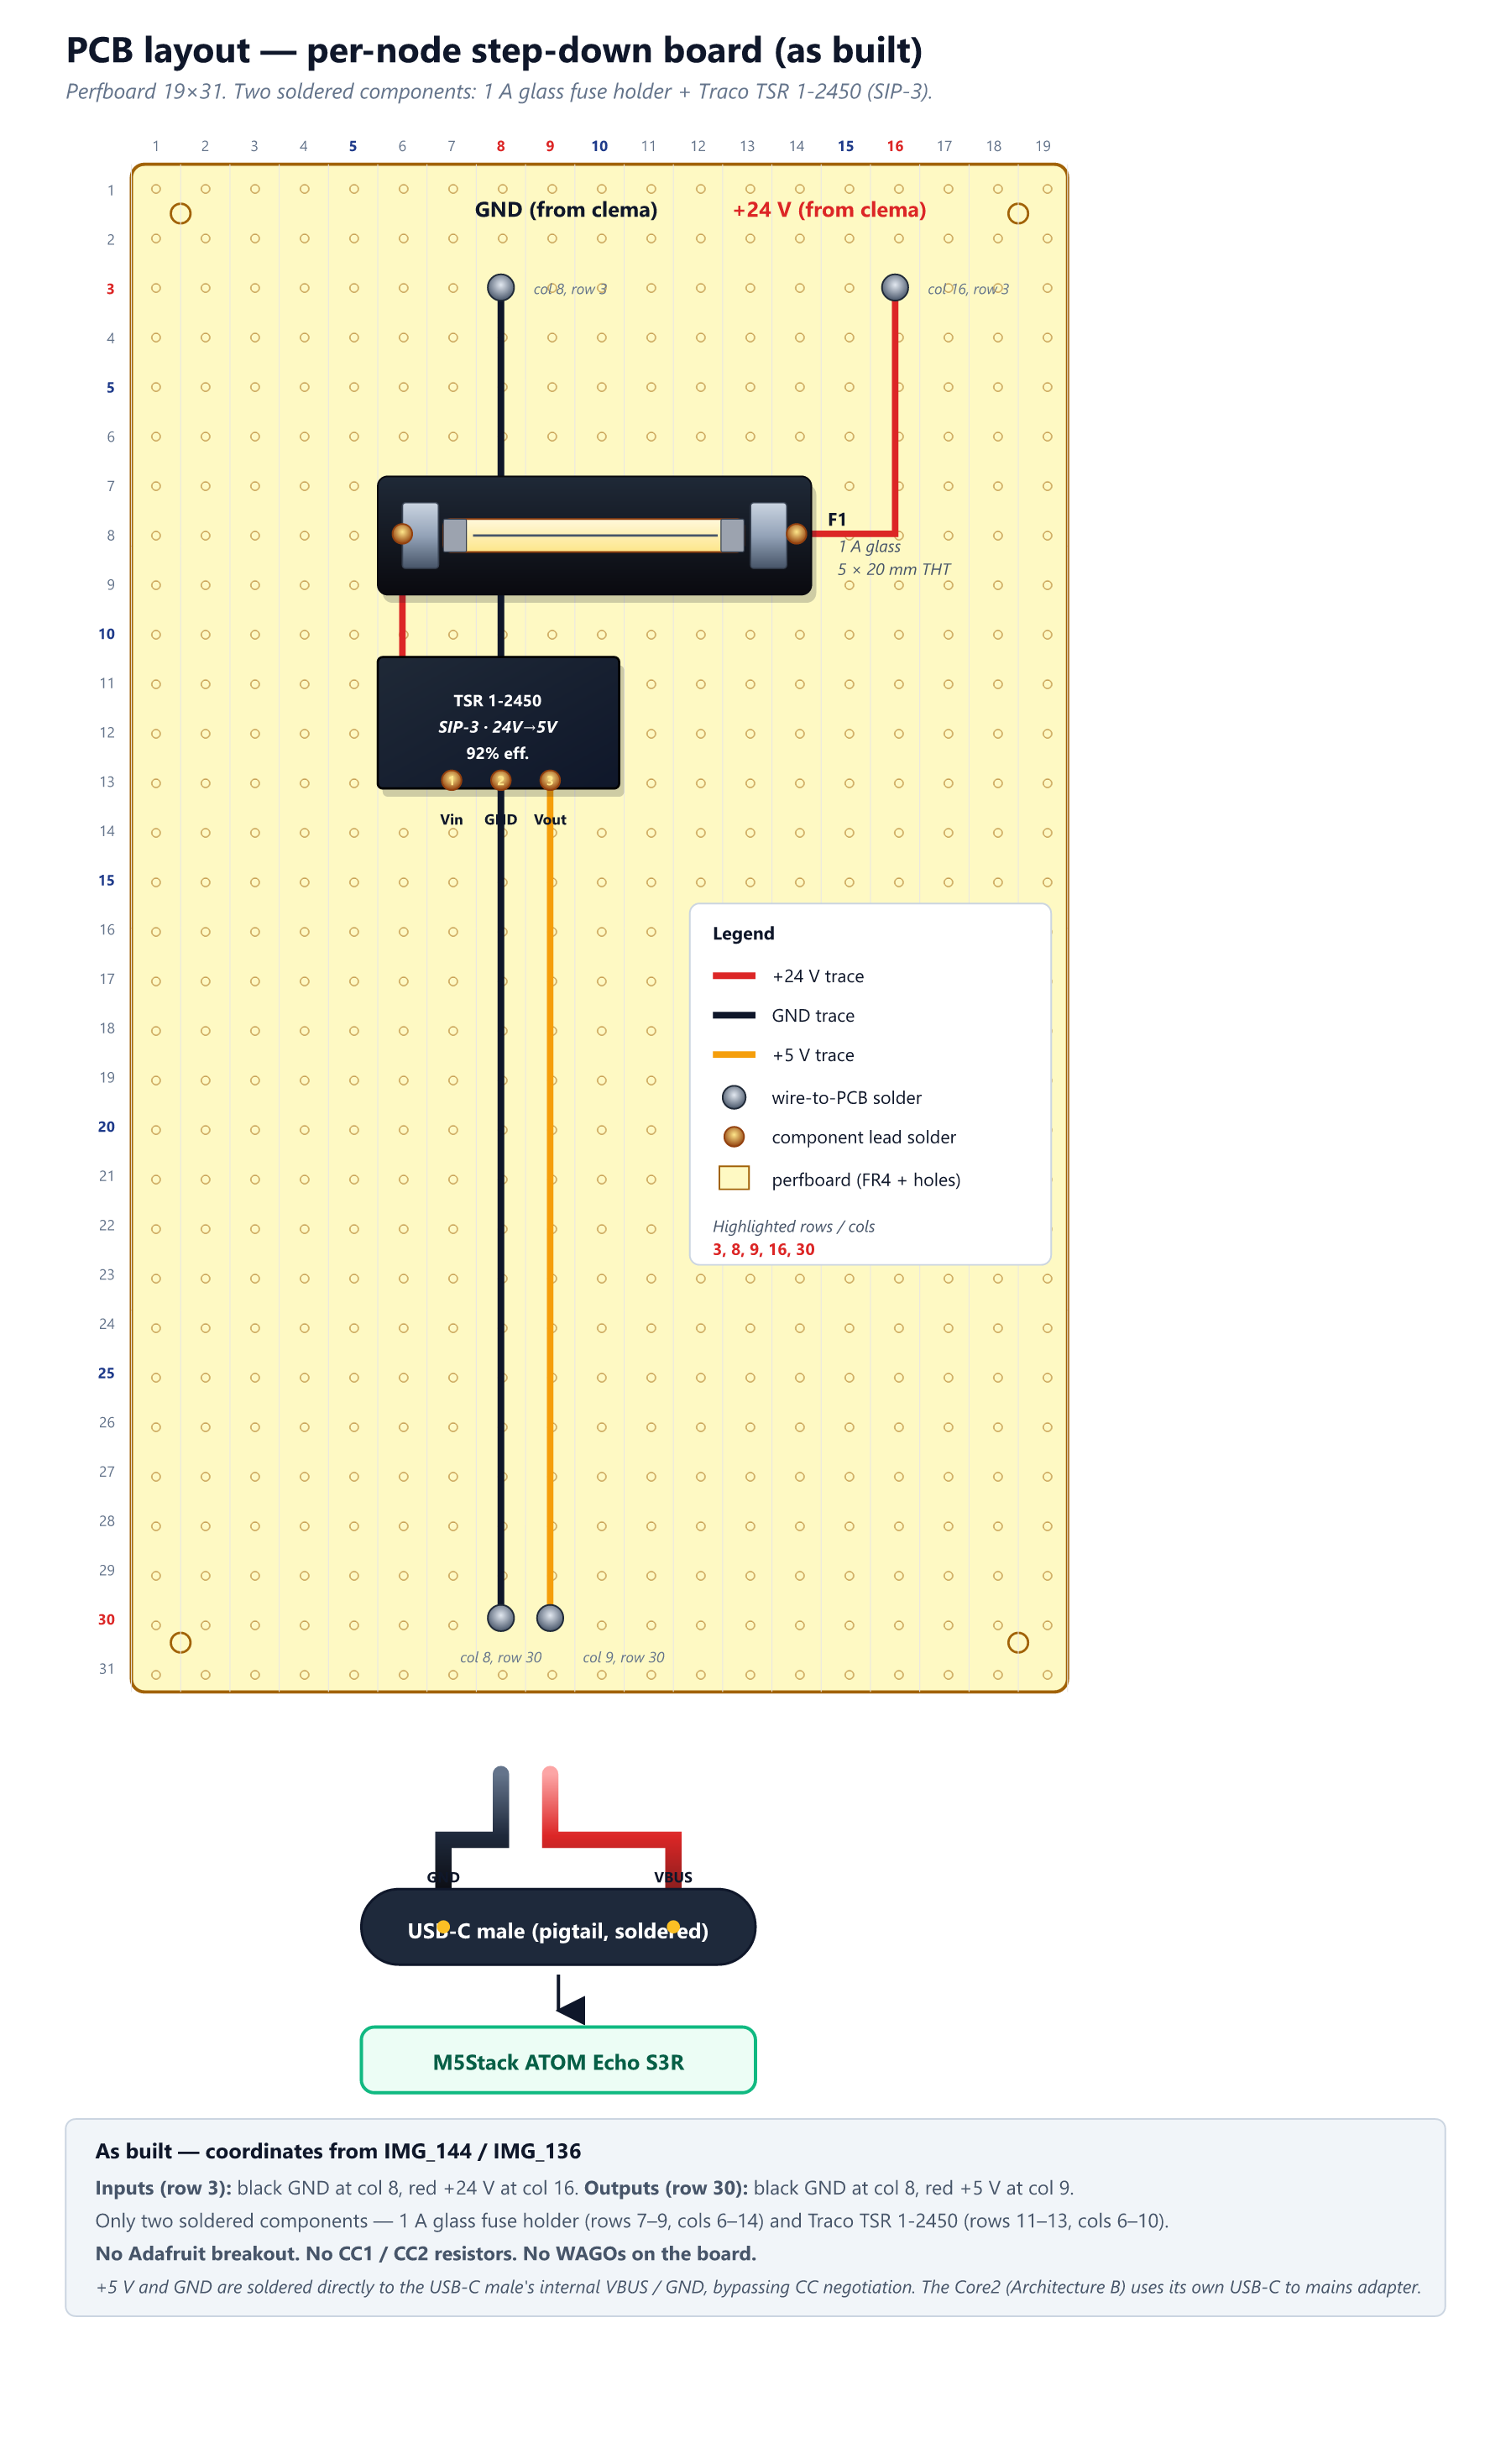
\includegraphics[width=0.78\textwidth]{schema_pcb_final.png}
\caption{Esquema as-built del PCB por nodo: bus de techo 24\,V $\to$ clema de electricista $\to$ fusible 1\,A $\to$ TSR 1-2450 $\to$ pigtail USB-C soldado $\to$ ATOM Echo S3R. El raíl GND pasa por fuera del TSR para evitar cruces con la huella del SIP-3.}
\label{fig:schema-pcb-final}
\end{figure}

Para contexto del proceso de dise\~no, la Figura \ref{fig:schema-pcb-rejected} muestra la revisi\'on previa descartada (con \emph{breakout} Adafruit USB-C y resistencias en CC1/CC2 conectadas err\'oneamente a $+5$\,V en lugar de a GND).

\begin{figure}[H]
\centering
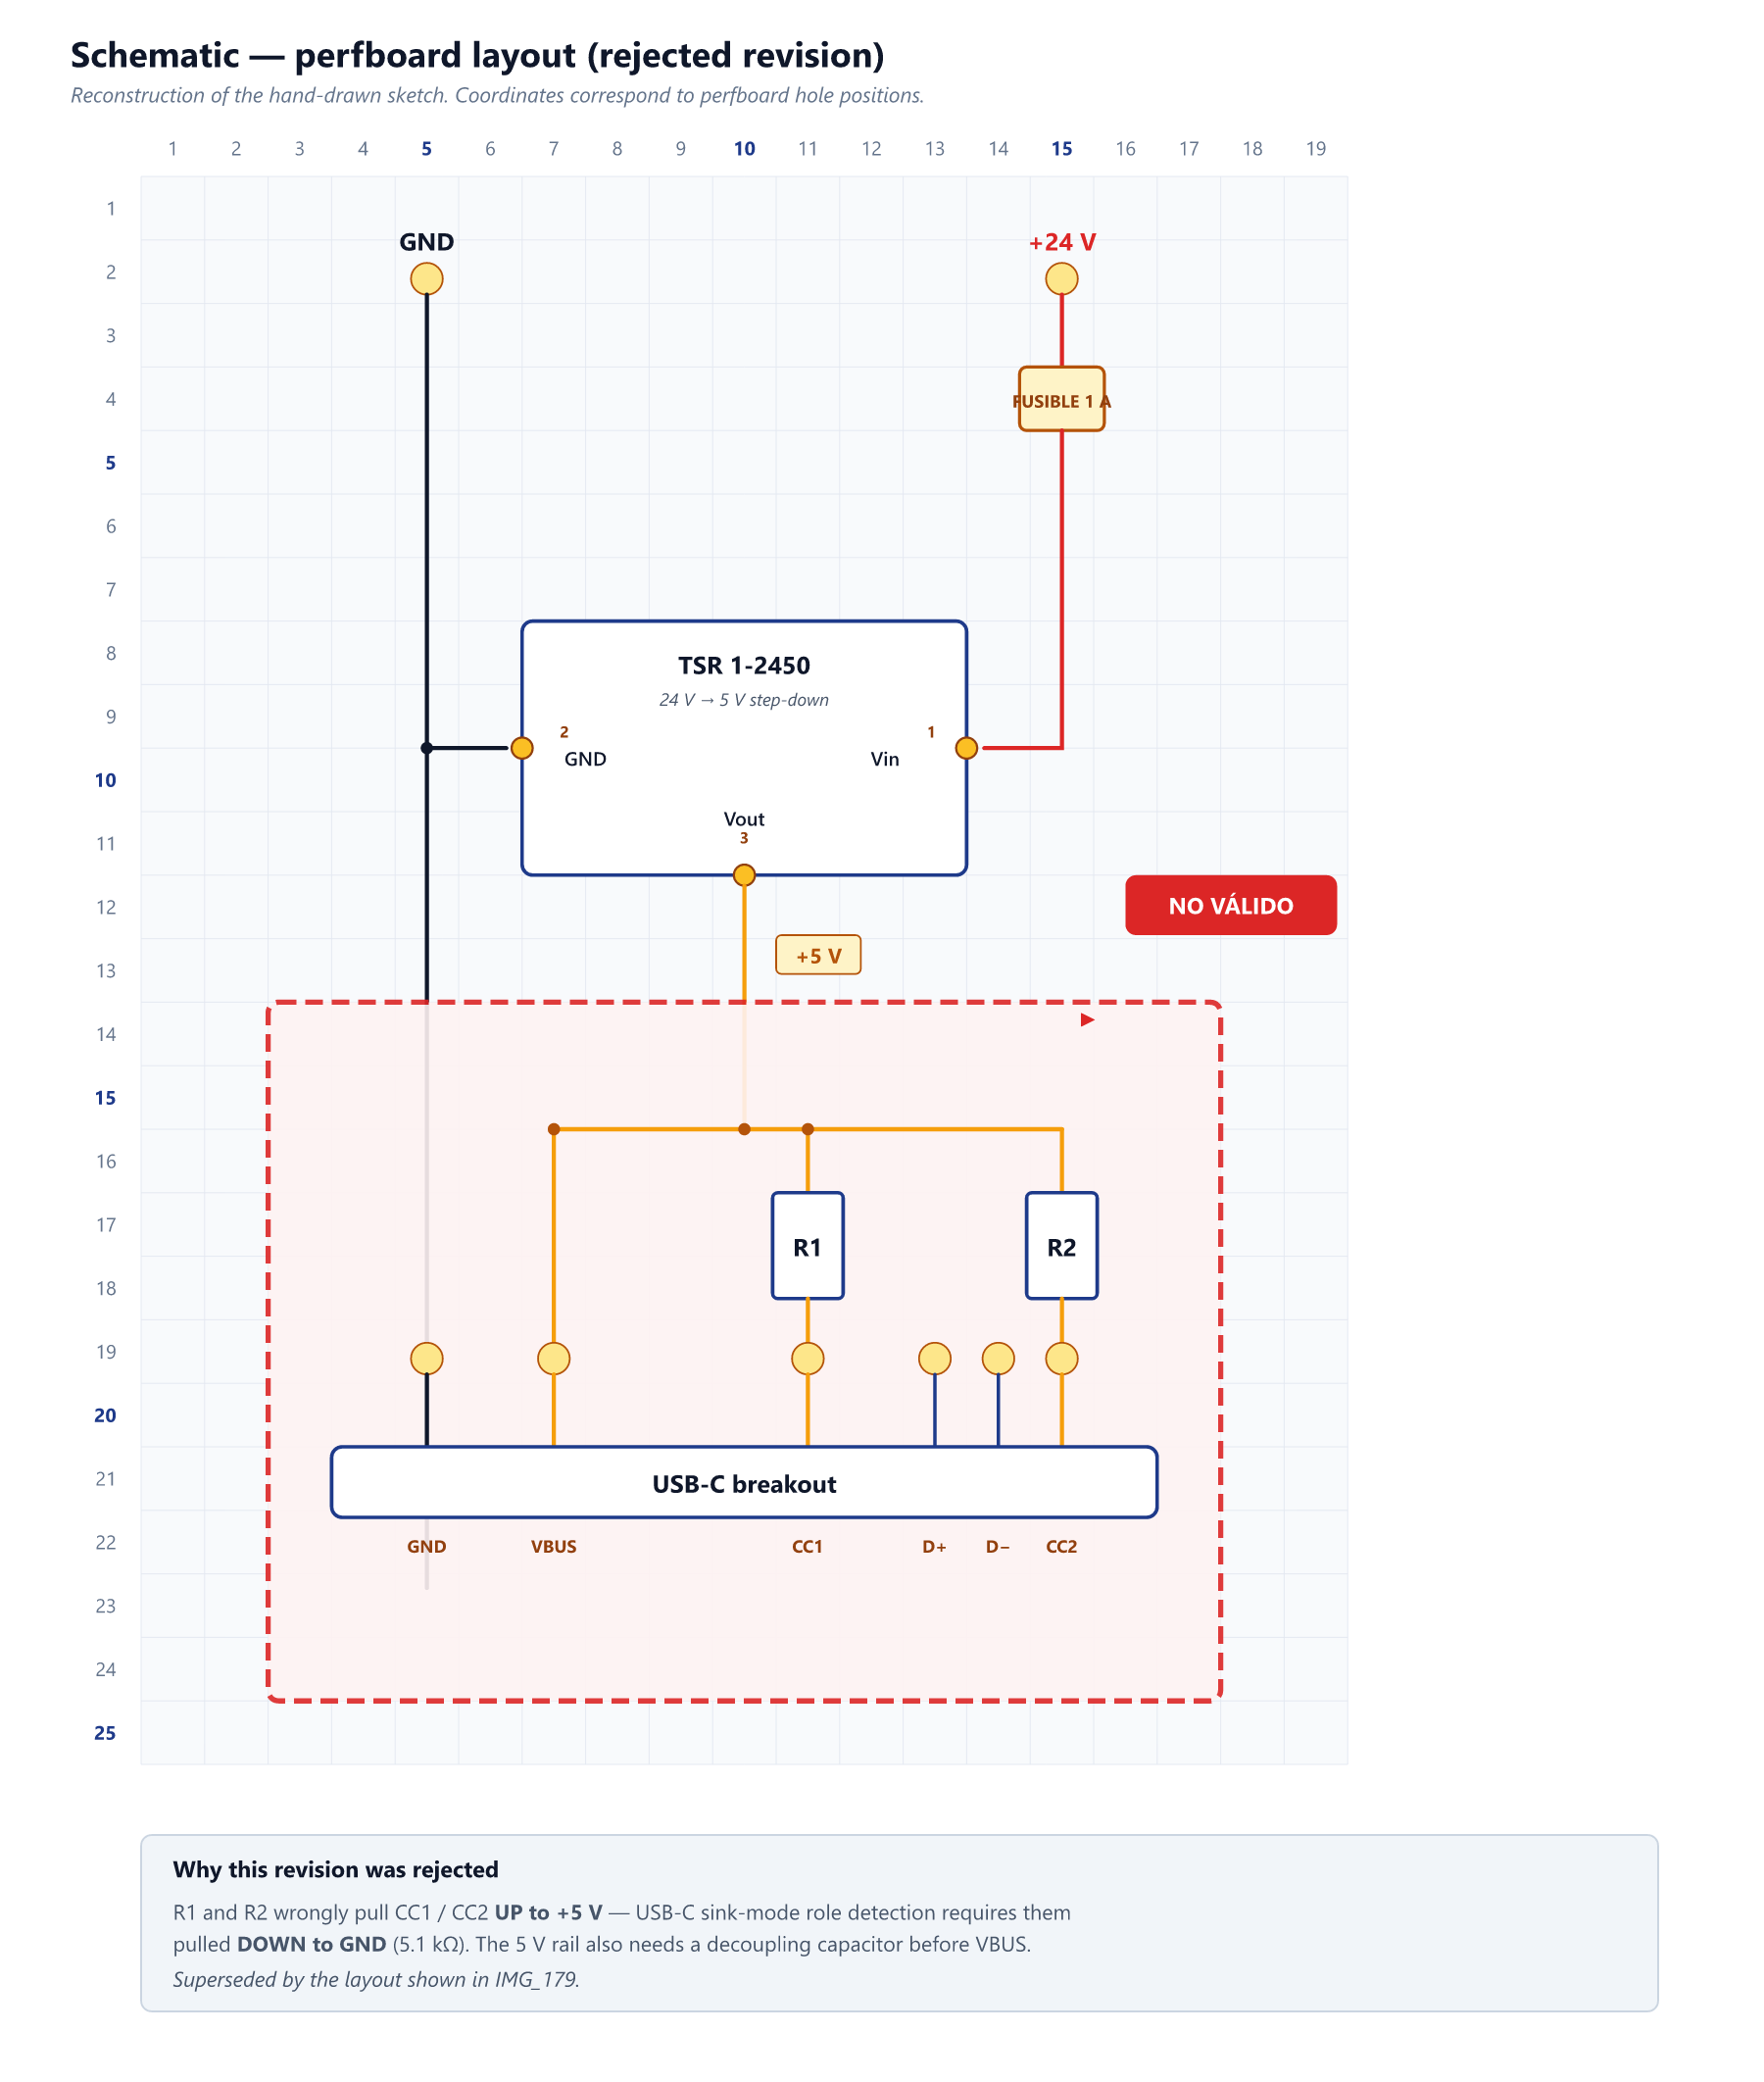
\includegraphics[width=0.7\textwidth]{schema_pcb_no_valido.png}
\caption{Revisi\'on descartada: \emph{pull-ups} en CC1/CC2 hacia $+5$\,V (cuando para modo \emph{sink} deber\'ian ser \emph{pull-downs} de 5{,}1\,k$\Omega$ a GND) y ausencia de capacidad de desacoplo antes de VBUS. Sustituida por la topolog\'ia de la Figura \ref{fig:schema-pcb-final}.}
\label{fig:schema-pcb-rejected}
\end{figure}

% =============================================================================
\chapter{Coeficientes del filtro A-weighting}

\begin{lstlisting}[language=C, caption={Coeficientes biquad para $f_s = 16{.}000$\,Hz}]
// Biquad 1: 2nd-order HP, fc=20.6Hz, Q=0.5
{ b0=0.991965,  b1=-1.983931, b2=0.991965,
  a1=-1.983906, a2=0.983946 }

// Biquad 2: 1st-order HP, fc=107.7Hz
{ b0=0.979286,  b1=-0.979286, b2=0.0,
  a1=-0.958573, a2=0.0 }

// Biquad 3: 1st-order HP, fc=737.9Hz
{ b0=0.873487,  b1=-0.873487, b2=0.0,
  a1=-0.746974, a2=0.0 }

// Ganancia de normalizacion 0 dB en 1 kHz
const float G_NORM = 1.24358f;
\end{lstlisting}

% =============================================================================
\chapter{Esquema de la base de datos}

\begin{lstlisting}[language=SQL, caption={Tabla raw \texttt{noise\_readings}}]
CREATE TABLE noise_readings (
    id         INTEGER PRIMARY KEY AUTOINCREMENT,
    room       TEXT    NOT NULL,
    mic        TEXT    NOT NULL DEFAULT 'mic_01',
    db_level   REAL    NOT NULL,
    peak_level REAL    NOT NULL,
    timestamp  INTEGER NOT NULL,
    created_at TEXT    DEFAULT (datetime('now'))
);

CREATE INDEX idx_room_mic_timestamp
    ON noise_readings (room, mic, timestamp DESC);
\end{lstlisting}

\begin{lstlisting}[language=SQL, caption={Tablas agregadas del rollup}]
CREATE TABLE noise_minute (
    room       TEXT    NOT NULL,
    mic        TEXT    NOT NULL,
    bucket_ts  INTEGER NOT NULL,  -- timestamp del minuto (mod 60)
    avg_db     REAL    NOT NULL,
    min_db     REAL    NOT NULL,
    max_db     REAL    NOT NULL,
    max_peak   REAL    NOT NULL,
    samples    INTEGER NOT NULL,
    PRIMARY KEY (room, mic, bucket_ts)
);

CREATE TABLE noise_hour (
    room       TEXT    NOT NULL,
    mic        TEXT    NOT NULL,
    bucket_ts  INTEGER NOT NULL,  -- timestamp de la hora (mod 3600)
    avg_db     REAL    NOT NULL,
    min_db     REAL    NOT NULL,
    max_db     REAL    NOT NULL,
    max_peak   REAL    NOT NULL,
    samples    INTEGER NOT NULL,
    PRIMARY KEY (room, mic, bucket_ts)
);
\end{lstlisting}

% =============================================================================
\chapter{Referencia r\'apida de comandos}

\begin{table}[H]
\centering
\rowcolors{2}{white}{BgGray}
\begin{tabularx}{\textwidth}{l X}
\toprule
\rowcolor{TableHead}
\textbf{Comando} & \textbf{Descripci\'on} \\ \midrule
\texttt{docker compose up -d}            & Arranque completo (backend + frontend + caddy + cloudflared) \\
\texttt{docker compose down}             & Detener todo \\
\texttt{docker compose logs -f backend}  & Ver logs del backend en vivo \\
\texttt{docker logs aulas-cloudflared}   & Mostrar URL p\'ublica del t\'unel \\
\texttt{cd backend \&\& npm start}       & Backend en local sin Docker \\
\texttt{cd frontend \&\& npm run dev}    & Frontend en local sin Docker \\
\texttt{cd simulator \&\& node simulate.js} & Simulador para demo sin hardware \\
\texttt{pio run -t upload}                & Flashear firmware al ESP32 (PlatformIO) \\
\texttt{pio device monitor}               & Monitor serie del nodo \\ \bottomrule
\end{tabularx}
\caption{Referencia r\'apida de comandos.}
\end{table}

% =============================================================================
\chapter{Glosario}

\begin{description}[style=nextline,leftmargin=2em]
    \item[A-weighting] Curva de ponderaci\'on frecuencial definida en IEC 61672 que modela la respuesta del o\'ido humano.
    \item[ABP] Aprendizaje Basado en Proyectos.
    \item[Biquad] Filtro digital IIR de segundo orden. Bloque b\'asico para construir filtros m\'as complejos.
    \item[Brown-out] Reinicio del microcontrolador por ca\'ida de tensi\'on de alimentaci\'on por debajo del umbral cr\'itico.
    \item[DAM] Desarrollo de Aplicaciones Multiplataforma. Ciclo formativo de grado superior.
    \item[dB(A)] Decibelios con ponderaci\'on A. Unidad de medida de nivel sonoro que tiene en cuenta la sensibilidad del o\'ido humano.
    \item[Direct Form II Transposed] Topolog\'ia de implementaci\'on de filtros digitales que minimiza el n\'umero de retardos y mejora la estabilidad num\'erica.
    \item[EAP-PEAP] \emph{Protected Extensible Authentication Protocol}. M\'etodo de autenticaci\'on para WPA2-Enterprise.
    \item[FCT] Formaci\'on en Centros de Trabajo.
    \item[I2S] \emph{Inter-IC Sound}. Protocolo de comunicaci\'on serie para audio digital.
    \item[IEC 61672] Norma internacional que regula los son\'ometros y la ponderaci\'on A/B/C/Z.
    \item[ISO 9241-6] Norma de ergonom\'ia que estipula los niveles m\'aximos de ruido en entornos de trabajo intelectual.
    \item[Mediana espacial] Mediana calculada sobre las lecturas simult\'aneas de varios sensores en el mismo instante. Robusta frente a sensores at\'ipicos.
    \item[MEMS] \emph{Micro-Electro-Mechanical Systems}. Tecnolog\'ia de fabricaci\'on de micr\'ofonos miniaturizados.
    \item[MQTT] \emph{Message Queuing Telemetry Transport}. Protocolo de mensajer\'ia ligero para IoT.
    \item[MTBF] \emph{Mean Time Between Failures}. Indicador de fiabilidad de un componente.
    \item[Nyquist] Mitad de la frecuencia de muestreo. L\'imite superior de las frecuencias representables sin alias.
    \item[OMS] Organizaci\'on Mundial de la Salud.
    \item[PDM] \emph{Pulse Density Modulation}. T\'ecnica de modulaci\'on usada por micr\'ofonos MEMS.
    \item[Quick Tunnel] Modalidad gratuita de Cloudflare Tunnel; URL p\'ublica HTTPS no permanente.
    \item[Rollup] Estrategia de agregaci\'on en cascada de datos hist\'oricos a granularidades crecientes.
    \item[RMS] \emph{Root Mean Square}. Valor eficaz de una se\~nal.
    \item[SMR] Sistemas Microinform\'aticos y Redes. Ciclo formativo de grado medio.
    \item[SPL] \emph{Sound Pressure Level}. Nivel de presi\'on sonora medido en decibelios.
    \item[WAGO] Marca de conectores el\'ectricos sin tornillo.
    \item[WAL] \emph{Write-Ahead Logging}. Modo de SQLite que permite lecturas concurrentes durante escrituras.
\end{description}

\end{document}
